\documentclass[11pt]{article}

\usepackage[utf8]{inputenc}
\usepackage[T1]{fontenc}
\usepackage[margin=2.6cm]{geometry}
\usepackage{amsmath,amssymb,amsthm}
\usepackage{enumerate}
\usepackage{comment}
\usepackage{times}
\usepackage[colorlinks,linkcolor=blue!55!black,citecolor=blue!55!black]{hyperref}

\usepackage{tikz}
\usetikzlibrary{arrows.meta,positioning,decorations.pathreplacing}
% No PSTricks and no auto-pst-pdf: every picture here is TikZ, so the collection
% builds with a plain `pdflatex`, without -shell-escape.

\input{../sty/macros}

% One source, two PDFs. Solutions are included by default; the student version
% is produced by defining \nosolutions before the file is read:
%   pdflatex -jobname=exercises "\def\nosolutions{}\documentclass[11pt]{article}

\usepackage[utf8]{inputenc}
\usepackage[T1]{fontenc}
\usepackage[margin=2.6cm]{geometry}
\usepackage{amsmath,amssymb,amsthm}
\usepackage{enumerate}
\usepackage{comment}
\usepackage{times}
\usepackage[colorlinks,linkcolor=blue!55!black,citecolor=blue!55!black]{hyperref}

\usepackage{tikz}
\usetikzlibrary{arrows.meta,positioning,decorations.pathreplacing}
% No PSTricks and no auto-pst-pdf: every picture here is TikZ, so the collection
% builds with a plain `pdflatex`, without -shell-escape.

\input{../sty/macros}

% One source, two PDFs. Solutions are included by default; the student version
% is produced by defining \nosolutions before the file is read:
%   pdflatex -jobname=exercises "\def\nosolutions{}\documentclass[11pt]{article}

\usepackage[utf8]{inputenc}
\usepackage[T1]{fontenc}
\usepackage[margin=2.6cm]{geometry}
\usepackage{amsmath,amssymb,amsthm}
\usepackage{enumerate}
\usepackage{comment}
\usepackage{times}
\usepackage[colorlinks,linkcolor=blue!55!black,citecolor=blue!55!black]{hyperref}

\usepackage{tikz}
\usetikzlibrary{arrows.meta,positioning,decorations.pathreplacing}
% No PSTricks and no auto-pst-pdf: every picture here is TikZ, so the collection
% builds with a plain `pdflatex`, without -shell-escape.

\input{../sty/macros}

% One source, two PDFs. Solutions are included by default; the student version
% is produced by defining \nosolutions before the file is read:
%   pdflatex -jobname=exercises "\def\nosolutions{}\documentclass[11pt]{article}

\usepackage[utf8]{inputenc}
\usepackage[T1]{fontenc}
\usepackage[margin=2.6cm]{geometry}
\usepackage{amsmath,amssymb,amsthm}
\usepackage{enumerate}
\usepackage{comment}
\usepackage{times}
\usepackage[colorlinks,linkcolor=blue!55!black,citecolor=blue!55!black]{hyperref}

\usepackage{tikz}
\usetikzlibrary{arrows.meta,positioning,decorations.pathreplacing}
% No PSTricks and no auto-pst-pdf: every picture here is TikZ, so the collection
% builds with a plain `pdflatex`, without -shell-escape.

\input{../sty/macros}

% One source, two PDFs. Solutions are included by default; the student version
% is produced by defining \nosolutions before the file is read:
%   pdflatex -jobname=exercises "\def\nosolutions{}\input{exercises.tex}"
% The Makefile target `exercises` builds both. Nothing has to be kept in sync.
\newif\ifsolutions
\solutionstrue
\ifdefined\nosolutions\solutionsfalse\fi

\newcounter{exercisecount}[section]
\renewcommand{\theexercisecount}{\thesection.\arabic{exercisecount}}
\newenvironment{exercise}
  {\par\medskip\refstepcounter{exercisecount}%
   \noindent\textbf{Exercise \theexercisecount.}\begin{itshape}}
  {\end{itshape}\par\medskip}

\ifsolutions
  \newenvironment{solution}
    {\par\nobreak\smallskip\noindent\textbf{Solution.}\par\nobreak\smallskip}
    {\par\medskip\hrule height 0pt\medskip}
\else
  \excludecomment{solution}
\fi

\newcommand{\WSv}{\mathrm{WS}}
\newcommand{\RPv}{\mathrm{RP}}
\newcommand{\EVv}{\mathrm{EV}}
\newcommand{\EEVv}{\mathrm{EEV}}
\newcommand{\EVPIv}{\mathrm{EVPI}}
\newcommand{\VSSv}{\mathrm{VSS}}

\title{Stochastic optimization\\[2mm] \Large Exercise collection%
\ifsolutions\\[2mm]\normalsize with solutions\fi}
\author{Fabian Bastin\\ \small Université de Montréal -- CIRRELT -- IVADO}
\date{}

\begin{document}

\maketitle

\noindent
This collection accompanies the lecture slides. Each exercise names the deck it
depends on.
\ifsolutions
This is the version \emph{with solutions}; the statements alone are in
\texttt{exercises.pdf}.
\else
This version holds the \emph{statements only}; the solutions are in
\texttt{exercises\_solutions.pdf}.
\fi

\medskip
\noindent
Sources are indicated exercise by exercise; several are adapted from Birge and
Louveaux, \emph{Introduction to Stochastic Programming}, 2nd edition, Springer,
2011.

\tableofcontents

%%%%%%%%%%%%%%%%%%%%%%%%%%%%%%%%%%%%%%%%%%%%%%%%%%%%%%%%%%%%%%%%%%%%%%%%%%%%%%
\section{Generalities}
%%%%%%%%%%%%%%%%%%%%%%%%%%%%%%%%%%%%%%%%%%%%%%%%%%%%%%%%%%%%%%%%%%%%%%%%%%%%%%

\begin{exercise}
(Deck~03.) Show that the value of the stochastic solution and the expected value
of perfect information are always non-negative.
\end{exercise}

\begin{solution}
Consider the general problem $\min_{x \in X} \EE[z(x,\bsxi)]$, and recall the
four quantities
\[
\RPv = \min_{x \in X} \EE[z(x,\bsxi)], \qquad
\WSv = \EE\left[ \min_{x \in X} z(x,\bsxi) \right], \qquad
\EVv = \min_{x \in X} z(x, \overline{\xi}), \quad \overline{\xi} = \EE[\bsxi],
\]
and
\[
\EEVv = \EE\left[ z\!\left(\overline{x}(\overline{\xi}), \bsxi\right) \right],
\qquad \overline{x}(\overline{\xi}) \in \arg\min_{x \in X} z(x,\overline{\xi}).
\]

\emph{A warning on $\EEVv$.} It is \textbf{not} $\EE[\EVv]$: $\EVv$ is a
deterministic number, so $\EE[\EVv] = \EVv$. $\EEVv$ is the expected cost of
\emph{using} the expected-value decision, the uncertainty being restored
afterwards. This is exactly what makes $\VSSv$ measure something.

\medskip
$\VSSv = \EEVv - \RPv \geq 0$. Since $\overline{x}(\overline{\xi}) \in X$, it is
one particular feasible point of the recourse problem, so
\[
\RPv = \min_{x \in X} \EE[z(x,\bsxi)] \leq \EE\left[z\!\left(\overline{x}(\overline{\xi}),\bsxi\right)\right] = \EEVv .
\]

\medskip
$\EVPIv = \RPv - \WSv \geq 0$. Let $x^*_{\RPv} \in \arg\min_{x \in X} \EE[z(x,\bsxi)]$.
For every realization $\xi$,
\[
z(x^*_{\RPv}, \xi) \geq \min_{x \in X} z(x,\xi),
\]
and taking expectations, which preserves inequalities,
\[
\RPv = \EE\left[z(x^*_{\RPv},\bsxi)\right] \geq \EE\left[\min_{x \in X} z(x,\bsxi)\right] = \WSv .
\]

\medskip
Both arguments have the same shape: a single decision that must serve every
realization can only be worse than a decision tailored to each one.
\end{solution}

%%%%%%%%%%%%%%%%%%%%%%%%%%%%%%%%%%%%%%%%%%%%%%%%%%%%%%%%%%%%%%%%%%%%%%%%%%%%%%
\section{Two-stage problems with recourse}
%%%%%%%%%%%%%%%%%%%%%%%%%%%%%%%%%%%%%%%%%%%%%%%%%%%%%%%%%%%%%%%%%%%%%%%%%%%%%%

\begin{exercise}
(Deck~01 and~03.) Consider the farmer problem of deck~01. Is its recourse
\emph{complete}? \emph{Relatively complete}? \emph{Simple}?
\end{exercise}

\begin{solution}
Write $t_1$, $t_2$, $t_3$ for the yields (tons per acre) of one scenario, $y_1$,
$y_2$ for the tons of wheat and corn bought, $w_1$, $w_2$ for the tons sold, and
$w_3$, $w_4$ for the tons of sugar beets sold at the high and at the low price.
Given the acreages $x$, the second stage is
\begin{align*}
\min_{y,w}\ & 238y_1 - 170w_1 + 210y_2 - 150w_2 - 36w_3 - 10w_4 \\
\text{s.t. } & t_1x_1 + y_1 - w_1 \geq 200, \qquad t_2x_2 + y_2 - w_2 \geq 240, \\
& w_3 + w_4 \leq t_3x_3, \qquad w_3 \leq 6000, \qquad y, w \geq 0.
\end{align*}
Adding slacks $s \geq 0$ and moving $x$ to the right-hand side,
\[
y_1 - w_1 - s_1 = 200 - t_1x_1, \quad
y_2 - w_2 - s_2 = 240 - t_2x_2, \quad
w_3 + w_4 + s_3 = t_3x_3, \quad
w_3 + s_4 = 6000,
\]
so that, with the columns ordered as $(y_1, y_2, w_1, w_2, w_3, w_4, s_1, s_2, s_3, s_4)$,
\[
W = \begin{pmatrix}
1 & 0 & -1 & 0 & 0 & 0 & -1 & 0 & 0 & 0 \\
0 & 1 & 0 & -1 & 0 & 0 & 0 & -1 & 0 & 0 \\
0 & 0 & 0 & 0 & 1 & 1 & 0 & 0 & 1 & 0 \\
0 & 0 & 0 & 0 & 1 & 0 & 0 & 0 & 0 & 1
\end{pmatrix}.
\]

\textbf{Not complete.} Rows 3 and 4 meet only columns with non-negative entries,
so every $z \in \operatorname{pos} W$ has $z_3 \geq 0$ and $z_4 \geq 0$.
Conversely any such $z$ is attained (take $w_3 = 0$, $s_4 = z_4$, $w_4 = z_3$,
$s_3 = 0$, and use $(y_1,w_1)$, $(y_2,w_2)$ for the first two rows, which are
unrestricted). Hence
$\operatorname{pos} W = \RR \times \RR \times \RR_+ \times \RR_+ \neq \RR^4$.

\textbf{Relatively complete.} We need $h(\xi) - T(\xi)x \in \operatorname{pos} W$
for every $x \in K_1 = \lbrace x \in \RR^3_+ \mid x_1+x_2+x_3 \leq 500 \rbrace$
and every scenario. Its third and fourth components are $t_3x_3$ and $6000$,
both non-negative since $x_3 \geq 0$ and the yields are positive. So
$K_1 \subseteq K_2$. Concretely, buying all the wheat and corn needed and selling
no sugar beets is feasible whatever the seeding decision and the yields ---
expensive, but feasible.

\textbf{Not simple.} Simple recourse requires $W = \begin{pmatrix} I & -I \end{pmatrix}$.
Here $W$ is $4 \times 10$ and $w_3$ appears in two rows, the quota coupling the
beet sales to the harvest.

\medskip
Completeness is read off $W$ alone and fails here on a technicality; relative
completeness --- the property that matters --- holds because every right-hand
side the model can produce lands in $\operatorname{pos} W$.
\end{solution}

\begin{exercise}
(Deck~03; Birge and Louveaux, p.~87.) Consider the second-stage program
\[
Q(x,\xi) = \min_y \lbrace y \mid \xi y = 1-x,\ y \geq 0 \rbrace,
\]
where $\bsxi$ follows a triangular distribution on $[0,1]$, i.e.\ $P[\bsxi \leq u] = u^2$.
\begin{enumerate}[(a)]
\item Is the recourse fixed? Why?
\item Express $K_2(\xi)$ for every $\xi \in [0,1]$.
\item Express $K_2$, $K_2^P$ and $\calQ$.
\end{enumerate}
\end{exercise}

\begin{solution}
\textbf{(a)} The recourse is \emph{not} fixed: here $W \equiv \bsxi$, which is
random. Moreover $\xi$ can take the value $0$, so the transformation
$y = (1-x)/\xi$ is not defined on all of $\Xi = [0,1]$. In terms of the cone,
\[
\operatorname{pos} W =
\begin{cases}
\lbrace 0 \rbrace & \text{if } \xi = 0, \\
\RR_+ & \text{if } \xi \neq 0.
\end{cases}
\]

\textbf{(b)} Two cases.
\emph{$\xi \in (0,1]$:} since $y \geq 0$ and $\xi > 0$, feasibility requires
$1-x \geq 0$, so $K_2(\xi) = \lbrace x \mid x \leq 1 \rbrace$, with
$Q(x,\xi) = (1-x)/\xi$ attained at $y^* = (1-x)/\xi$.
\emph{$\xi = 0$:} no $y$ satisfies $0 \cdot y = 1-x$ unless $x = 1$, so
$K_2(0) = \lbrace 1 \rbrace$.

\textbf{(c)} Therefore
\[
K_2^P = \lbrace x \mid x \leq 1 \rbrace \cap \lbrace 1 \rbrace = \lbrace 1 \rbrace,
\]
while, since $P[\bsxi = 0] = 0$ and the density is $f(\xi) = 2\xi$,
\[
\calQ(x) = \int_0^1 \frac{1-x}{\xi}\, 2\xi \, d\xi = 2(1-x), \qquad \forall x \leq 1,
\]
so $K_2 = \lbrace x \mid x \leq 1 \rbrace$ and $K_2^P \subsetneq K_2$.

\medskip
The difference is that a point leaves $K_2^P$ as soon as it is infeasible for
\emph{one} value of $\xi$, whatever its probability, whereas $K_2$ ignores
infeasibilities occurring with probability zero. Recall that for a program with
a \emph{fixed} recourse --- not the case here --- and $\bsxi$ with finite
second-order moments, we would have had $K_2 = K_2^P$.
\end{solution}

\begin{exercise}
(Deck~03.) Consider the second-stage program
\begin{align*}
\min_y\ & 2y_1+y_2\\
\text{s.t. } & y_1 - y_2 \leq 2-\bsxi x_1,\\
& y_2 \leq x_2,\\
& y_1, y_2 \geq 0.
\end{align*}
Find $K_2(\xi)$ and $K_2$ when (a) $\bsxi \sim U[0,1]$; (b) $\bsxi \sim \text{Poisson}(\lambda)$, $\lambda > 0$.
Which properties do you expect of $K_2$? Is the recourse simple or complete? If
not, under which conditions would it be relatively complete?
\end{exercise}

\begin{solution}
\textbf{The elementary set.} $y_2 \geq 0$ and $y_2 \leq x_2$ force $x_2 \geq 0$.
The first constraint then reads $y_1 \leq 2 - \xi x_1 + y_2$, and the largest
admissible right-hand side is obtained at $y_2 = x_2$; a feasible $y_1 \geq 0$
exists if and only if $2 - \xi x_1 + x_2 \geq 0$. Hence
\[
K_2(\xi) = \lbrace x \mid x_2 \geq 0,\ \xi x_1 \leq 2+x_2 \rbrace
= \lbrace x \mid x_2 \geq \max(0, \xi x_1 - 2) \rbrace .
\]

\textbf{(a) $\bsxi \sim U[0,1]$}, $\Xi = [0,1]$. The recourse is fixed ($\bsxi$
enters only through $T(\bsxi)$) and the distribution has finite second-order
moments, so $K_2 = K_2^s = K_2^P = \bigcap_{\xi \in \Xi} K_2(\xi)$.
For $x_1 \geq 0$ and $\xi \leq 1$, $\xi x_1 \leq x_1$, so
$x \in K_2(1) \Rightarrow x \in K_2(\xi)$; for $x_1 < 0$, $\xi x_1 \leq 0 \leq 2+x_2$
always. In both cases $K_2(1) \subseteq K_2(\xi)$ for every $\xi \in \Xi$: the
intersection is reached at $\xi = 1$ and
\[
K_2 = \lbrace x \mid x_2 \geq 0,\ x_1 \leq 2+x_2 \rbrace .
\]

\textbf{(b) $\bsxi \sim \text{Poisson}(\lambda)$}, $\Xi = \lbrace 0,1,2,\ldots\rbrace$
unbounded. If $x_1 > 0$ then $\xi x_1$ is unbounded above and no $x_2$ absorbs
it; if $x_1 \leq 0$ then $\xi x_1 \leq 0 \leq 2+x_2$. Hence
$K_2 = \lbrace x \mid x_1 \leq 0,\ x_2 \geq 0 \rbrace$.

\textbf{Expected properties.} Each $K_2(\xi)$ is an intersection of two
half-spaces, hence closed and convex, and so is $K_2$. This is no accident: with
a fixed recourse $x \in K_2(\xi) \iff h(\xi)-T(\xi)x \in \operatorname{pos} W$,
and $\operatorname{pos} W$ is a closed convex cone. With a finite support $K_2$
would moreover be polyhedral; here $\Xi$ is infinite, yet both answers happen to
be polyhedral.

\textbf{Type of recourse.} Putting the program in standard form with surplus
variables $s_1, s_2 \geq 0$,
\[
y_1 - y_2 + s_1 = 2 - \xi x_1, \qquad y_2 + s_2 = x_2,
\qquad
W = \begin{pmatrix} 1 & -1 & 1 & 0 \\ 0 & 1 & 0 & 1 \end{pmatrix}.
\]
The recourse is \emph{not simple} ($W$ is not $\begin{pmatrix} I & -I\end{pmatrix}$),
and \emph{not complete}: the second row involves only non-negative coefficients,
so $z_2 < 0$ is unreachable and $\operatorname{pos} W = \RR \times \RR_+ \neq \RR^2$.
It is \emph{relatively complete} exactly when $K_1 \subseteq K_2$, i.e.\ when the
first stage already enforces $x_2 \geq 0$ together with $x_1 \leq 2+x_2$ in
case~(a), or $x_1 \leq 0$ in case~(b). If the first stage merely requires
$x \geq 0$, then
\[
\text{(a)}\quad K_1 \cap K_2 \subseteq \lbrace x \geq 0 \mid x_1 \leq 2+x_2 \rbrace,
\qquad
\text{(b)}\quad K_1 \cap K_2 \subseteq \lbrace x \mid x_1 = 0,\ x_2 \geq 0 \rbrace .
\]
Relative completeness is plausible in the first case and very restrictive in the
second: an unbounded support is far less forgiving, since \emph{every}
realization has to be survived.
\end{solution}

\begin{exercise}
(Deck~03; Birge and Louveaux, p.~102.) Consider the second-stage program
\begin{align*}
\min_y\ & 2y_1+y_2\\
\text{s.t. } & y_1 + y_2 \geq 1-x_1,\\
& y_1 \geq \bsxi - x_1-x_2,\\
& y_1, y_2 \geq 0.
\end{align*}
Show that this program has a complete recourse when $\bsxi$ has a finite expectation.
\end{exercise}

\begin{solution}
\textbf{A direct argument.} Completeness asks that for every right-hand side
$(z_1, z_2)$ there exist $y_1, y_2 \geq 0$ with $y_1 + y_2 \geq z_1$ and
$y_1 \geq z_2$. Taking $y_1 = \max\lbrace 0, z_2 \rbrace$ satisfies the second,
and $y_2 = \max\lbrace 0, z_1 - y_1 \rbrace$ the first; both are non-negative.

\textbf{Through $\operatorname{pos} W$.} The standard characterisation requires
$Wy = z$ with $y \geq 0$, and is stated for equalities: showing that $Wy \geq z$
is solvable is \emph{not} the same statement. So bring the program to the
standard form first, with surplus variables $s \geq 0$:
\[
y_1 + y_2 - s_1 = 1-x_1, \qquad y_1 - s_2 = \xi - x_1 - x_2,
\qquad
W = \begin{pmatrix} 1 & 1 & -1 & 0 \\ 1 & 0 & 0 & -1 \end{pmatrix}.
\]
The second row leaves $y_1$ free to absorb the sign of $z_2$:
\[
\begin{cases}
y_1 = z_2,\ s_2 = 0 & \text{if } z_2 \geq 0,\\
y_1 = 0,\ s_2 = -z_2 & \text{otherwise.}
\end{cases}
\]
The first row then reads $y_2 - s_1 = z_1 - y_1$. If $z_2 \geq 0$, then
$y_2 - s_1 = z_1 - z_2$ and we take
\[
\begin{cases}
y_2 = z_1-z_2,\ s_1 = 0 & \text{if } z_1-z_2 \geq 0,\\
y_2 = 0,\ s_1 = z_2-z_1 & \text{otherwise;}
\end{cases}
\]
if $z_2 < 0$, then $y_1 = 0$, $y_2 - s_1 = z_1$, and it suffices to choose
\[
\begin{cases}
y_2 = z_1,\ s_1 = 0 & \text{if } z_1 \geq 0,\\
y_2 = 0,\ s_1 = -z_1 & \text{otherwise.}
\end{cases}
\]
Every $z \in \RR^2$ is reached, so $\operatorname{pos} W = \RR^2$ and the
recourse is complete.

\textbf{The hypothesis on $\EE[\bsxi]$ played no role}, and could not have:
completeness involves only $W$, which is fixed. The statement is copied from
Birge and Louveaux, where the hypothesis is superfluous at this point. In
particular it is \emph{not} what gives $K_2 = \RR^2$ --- completeness alone does.

What a finite expectation buys is the \emph{finiteness} of the recourse. Deck~03
uses exactly this $W$ with $P[\bsxi = 2^n] = 2^{-(n+1)}$, $n = 0,1,2,\ldots$, for
which $\EE[\bsxi] = +\infty$, to exhibit a problem where the recourse is complete
--- hence $K_2 = \RR^2$ --- while $\calQ(x) = +\infty$ everywhere, so
$K_2^s = \emptyset$. Complete recourse and finite recourse are two different
things.
\end{solution}

\begin{exercise}
(Deck~03.) A company must order a quantity $x$ of a product to meet a demand $d$
that is unknown at the time of ordering. The unit ordering cost is $c > 0$. If
$d > x$, a penalty $b \geq 0$ is incurred per unit of unmet demand; if $d < x$,
a holding cost $h$ is incurred per surplus unit.
\begin{enumerate}[(a)]
\item Formulate the problem as a two-stage stochastic program.
\item Is the recourse simple, complete, relatively complete?
\item What can be expected of the first-stage solution when $b < c$?
\end{enumerate}
\end{exercise}

\begin{solution}
\textbf{(a)} The first stage is the order; the second stage settles the
discrepancy between $x$ and the realized demand:
\[
\min_{x \geq 0}\ cx + \EE_{\bsd}[Q(x,\bsd)],
\qquad
Q(x,d) = \min_{y^+,y^- \geq 0} \lbrace by^+ + hy^- \mid y^+ - y^- = d-x \rbrace .
\]

\textbf{(b)} Here $W = \begin{pmatrix} 1 & -1 \end{pmatrix}$, so the recourse is
\emph{simple}, hence also complete and relatively complete. The finiteness
condition of the simple-recourse theorem reads $b + h \geq 0$, satisfied as soon
as both costs are non-negative.

\textbf{(c)} With $b < c$, an extra ordered unit costs more than the penalty it
avoids. Formally, the objective $cx + \EE[b(\bsd-x)^+ + h(x-\bsd)^+]$ has
right derivative at $x$ equal to $c - b\,P[\bsd > x] + h\,P[\bsd < x] \geq c - b > 0$,
so the objective is strictly increasing and $x^* = 0$: the company orders
nothing and pays the penalty.
\end{solution}

\begin{exercise}
(Deck~03.) A good $X$ must be produced before its demand is known. Each unit
produced costs \$2. Demand is discrete, taking the values $D_s$ with
probabilities $p_s$, $s = 1,\ldots,S$. Demand can also be met by buying from an
external supplier at \$3 per unit, once it has been observed. How much should be
produced now? Formulate the problem as a two-stage stochastic program minimizing
the expected production cost.
\end{exercise}

\begin{solution}
Let $x \geq 0$ be the number of units produced at the first stage, and
$y_s \geq 0$ the number bought from the external supplier in scenario $s$. Demand
is met when $x + y_s \geq D_s$, so
\begin{align*}
\min\ & 2x + \sum_{s=1}^S p_s\, 3 y_s \\
\text{s.t. } & x + y_s \geq D_s, \quad s = 1,\ldots,S, \\
& x \geq 0, \quad y_s \geq 0, \quad s = 1,\ldots,S.
\end{align*}
The second stage decomposes scenario by scenario, with $y_s = (D_s - x)^+$, so
the model is a simple-recourse one: producing is cheaper than outsourcing, but
must be committed to before the demand is known.
\end{solution}

\begin{exercise}
(Deck~03; Higle, \emph{Tutorials in Operations Research}, INFORMS, 2005.)
The Dakota Furniture Company makes desks, tables and chairs. Each item consumes
lumber and two kinds of skilled labour, finishing and carpentry:

\begin{center}
\begin{tabular}{|l|c|c|c|c|}
\hline
Resource & Cost & Desk & Table & Chair \\
\hline
Lumber (board ft.) & \$2 & 8 & 6 & 1 \\
Finishing (hours)  & \$4 & 4 & 2 & 1.5 \\
Carpentry (hours)  & \$5.2 & 2 & 1.5 & 0.5 \\
\hline
Selling price & & \$60 & \$40 & \$10 \\
\hline
\end{tabular}
\end{center}

Resources must be acquired before the demand is known. Three equally structured
demand scenarios are considered, with probabilities $0.3$, $0.4$ and $0.3$:

\begin{center}
\begin{tabular}{|l|c|c|c|}
\hline
Scenario & Desks & Tables & Chairs \\
\hline
Low ($p = 0.3$)         & 50  & 20  & 200 \\
Most likely ($p = 0.4$) & 150 & 110 & 225 \\
High ($p = 0.3$)        & 250 & 250 & 500 \\
\hline
\end{tabular}
\end{center}

Formulate the problem as a two-stage stochastic program maximizing the expected
profit. Only the formulation is asked.
\end{exercise}

\begin{solution}
Treat it as a resource-allocation problem. First stage: $x_1$ board feet of
lumber, $x_2$ finishing hours, $x_3$ carpentry hours. Second stage: $y_1$ desks,
$y_2$ tables, $y_3$ chairs produced once the demand is known.
\[
\min_{x \geq 0}\ 2x_1 + 4x_2 + 5.2x_3 + \EE_{\bsxi}[Q(x,\bsxi)],
\]
with
\begin{align*}
Q(x,\xi) = \min_y\ & -60y_1 - 40y_2 - 10y_3 \\
\text{s.t. } & 8y_1 + 6y_2 + y_3 \leq x_1, \\
& 4y_1 + 2y_2 + 1.5y_3 \leq x_2, \\
& 2y_1 + 1.5y_2 + 0.5y_3 \leq x_3, \\
& y_i \leq d_i(\xi),\ i = 1,2,3, \qquad y \geq 0 .
\end{align*}
Maximizing profit is minimizing its negative, hence the signs in $Q$. With the
three scenarios,
\[
\EE_{\bsxi}[Q(x,\bsxi)] = 0.3\,Q(x,\xi_1) + 0.4\,Q(x,\xi_2) + 0.3\,Q(x,\xi_3),
\]
where $d(\xi_1) = (50,20,200)$, $d(\xi_2) = (150,110,225)$ and
$d(\xi_3) = (250,250,500)$.
\end{solution}

\begin{exercise}
(Deck~03; Birge and Louveaux, p.~142.) Consider
\begin{align*}
\min_x\ & x_1 + 4x_2 + \EE_{\bsxi}[Q(x,\bsxi)] \\
\text{s.t. } & x_1 + x_2 = 1, \quad x \geq 0,
\end{align*}
with
\begin{align*}
Q(x,\xi) = \min_y\ & y_1 + 10y_2 + 10y_3 \\
\text{s.t. } & y_1 + y_2 - y_3 = \xi + x_1 - 2x_2, \\
& y_1 \leq 2, \qquad y \geq 0,
\end{align*}
and $\bsxi \sim U[1,3]$.
\begin{enumerate}[(a)]
\item Is the recourse fixed, simple, complete, relatively complete? Answer true
or false for each, with a brief justification.
\item For given $x$ and $\xi$, show, by discussing the value of $\xi + x_1 - 2x_2$, that
\[
y^*(x,\xi) =
\begin{cases}
y_1 = \xi + x_1 - 2x_2,\ y_2 = y_3 = 0 & \text{if } 0 \leq \xi + x_1 - 2x_2 \leq 2,\\
y_1 = 2,\ y_2 = \xi + x_1 - 2x_2 - 2,\ y_3 = 0 & \text{if } \xi + x_1 - 2x_2 > 2,\\
y_3 = 2x_2 - \xi - x_1,\ y_1 = y_2 = 0 & \text{if } \xi + x_1 - 2x_2 < 0.
\end{cases}
\]
\item Which expected property of $Q(x,\xi)$ does $y^*(x,\xi)$ confirm?
\item Is $\calQ(x) = \EE_{\bsxi}[Q(x,\bsxi)]$ differentiable? Why?
\item Express $K_1$, $K_2(\xi)$, $K_2^P$ and $K_2$.
\item Give the deterministic equivalent (extensive form) of the discretized
problem where $\bsxi$ takes the values $1$, $2$, $3$.
\end{enumerate}
\end{exercise}

\begin{solution}
\textbf{(a)} Adding a slack $y_4$ to the second constraint puts the second stage
in standard form,
\[
y_1 + y_2 - y_3 = \xi + x_1 - 2x_2, \qquad y_1 + y_4 = 2,
\qquad
W = \begin{pmatrix} 1 & 1 & -1 & 0 \\ 1 & 0 & 0 & 1 \end{pmatrix}.
\]
\emph{Fixed}: true, $W$ does not depend on $\xi$.
\emph{Simple}: false, $W$ is not of the form $\begin{pmatrix} I & -I\end{pmatrix}$.
\emph{Complete}: false --- the second row reads $y_1 + y_4 = z_2$ with
$y_1, y_4 \geq 0$, so no $z_2 < 0$ is reachable.
\emph{Relatively complete}: true. For any $x \in K_1$ and any $\xi$, the point
\[
y_1 = 0, \quad y_2 = (\xi + x_1 - 2x_2)^+, \quad y_3 = (-\xi - x_1 + 2x_2)^+, \quad y_4 = 2
\]
is feasible, the second component of the right-hand side being the constant $2 \geq 0$.

\textbf{(b)} Write $d = \xi + x_1 - 2x_2$. If $d < 0$, the only feasible extreme
point is $y_1 = y_2 = 0$, $y_3 = -d$, $y_4 = 2$, hence optimal. If $d \geq 0$,
an extreme point has $y_3 = 0$ and $y_1 + y_2 = d$ with $y_1 \leq 2$. Since the
cost of $y_1$ is $1$ and that of $y_2$ is $10$, $y_1$ is pushed as far as
possible: $y_1 = \min\lbrace d, 2 \rbrace$. This splits into $d \leq 2$, giving
$y_1 = d$, $y_2 = 0$, and $d \geq 2$, giving $y_1 = 2$, $y_2 = d-2$, as announced.

\textbf{(c)} $Q(\cdot,\xi)$ is convex and piecewise linear in the first-stage
decision $x$: the three regimes above are the three linear pieces, with
breakpoints where $d = 0$ and $d = 2$.

\textbf{(d)} Yes. $\bsxi$ is continuous with an absolutely continuous
distribution and finite second-order moments, so $\calQ$ is differentiable on the
interior of $K_2$: integrating over $\xi$ smooths away the kinks of each
$Q(\cdot,\xi)$.

\textbf{(e)} Directly from the statement,
$K_1 = \lbrace x \mid x_1 + x_2 = 1,\ x \geq 0 \rbrace$.
From (b), the second stage is feasible whatever $d$, so
$K_2(\xi) = \RR^2$ for every $\xi$, and therefore
$K_2^P = \bigcap_{\xi \in \Xi} K_2(\xi) = \RR^2$ and $K_2 = \RR^2$ as well.
In particular $K_1 \subseteq K_2$, confirming (a).

\textbf{(f)} With $\xi_1 = 1$, $\xi_2 = 2$, $\xi_3 = 3$ and $p_i = 1/3$,
\begin{align*}
\min\ & x_1 + 4x_2 + \sum_{i=1}^3 p_i\left(y_{1i} + 10y_{2i} + 10y_{3i}\right) \\
\text{s.t. } & x_1 + x_2 = 1, \\
& y_{1i} + y_{2i} - y_{3i} = \xi_i + x_1 - 2x_2, \quad i = 1,2,3, \\
& y_{1i} \leq 2, \quad i = 1,2,3, \\
& x \geq 0, \quad y_{1i}, y_{2i}, y_{3i} \geq 0, \quad i = 1,2,3.
\end{align*}
\end{solution}

%%%%%%%%%%%%%%%%%%%%%%%%%%%%%%%%%%%%%%%%%%%%%%%%%%%%%%%%%%%%%%%%%%%%%%%%%%%%%%
\section{Decomposition methods}
%%%%%%%%%%%%%%%%%%%%%%%%%%%%%%%%%%%%%%%%%%%%%%%%%%%%%%%%%%%%%%%%%%%%%%%%%%%%%%

\begin{exercise}
(Deck~04.) Consider
\begin{align*}
\min\ & 100x_1 + 150x_2 + \EE_{\bsxi}[q_1y_1 + q_2y_2] \\
\text{s.t. } & x_1 + x_2 \leq 120, \\
& 6y_1 + 10y_2 \leq 60x_1, \qquad 8y_1 + 5y_2 \leq 80x_2, \\
& y_1 \leq d_1, \qquad y_2 \leq d_2, \\
& x_1 \geq 40,\ x_2 \geq 20, \qquad y_1, y_2 \geq 0,
\end{align*}
under two scenarios $\bsxi = (d_1, d_2, q_1, q_2)$: $\xi_1 = (500, 100, -24, -28)$
with probability $p_1 = 0.4$, and $\xi_2 = (300, 300, -28, -32)$ with
probability $p_2 = 0.6$.

Run the first iteration of the single-cut $L$-shaped method, showing that the
second-stage solutions are respectively $y^* = (137.5, 100)$ and
$y^* = (80, 192)$. To obtain the dual solutions, use complementary slackness: a
dual variable can be non-zero only if the associated primal constraint is active.
\end{exercise}

\begin{solution}
\textbf{Master problem.} With no cut yet,
$\min \lbrace 100x_1 + 150x_2 \mid x_1 + x_2 \leq 120,\ x_1 \geq 40,\ x_2 \geq 20 \rbrace$,
whose optimal solution is immediately $x^1 = (40, 20)$, so $60x_1 = 2400$ and
$80x_2 = 1600$.

Since $x_1, x_2 \geq 0$ makes the second stage always feasible, the recourse is
relatively complete and no feasibility cut is needed.

\textbf{First scenario.}
$\min -24y_1 - 28y_2$ s.t. $6y_1 + 10y_2 \leq 2400$, $8y_1 + 5y_2 \leq 1600$,
$y_1 \leq 500$, $y_2 \leq 100$, $y \geq 0$.
We cannot have $y_1 = 500$, as the second constraint would be violated.
Setting $y_2 = 100$,
\[
y_1 = \min\left\lbrace \frac{2400-1000}{6},\ \frac{1600-500}{8} \right\rbrace
= \min\left\lbrace \frac{1400}{6},\ \frac{1100}{8} \right\rbrace
= \min\left\lbrace 233.33,\ 137.5 \right\rbrace = 137.5 .
\]
The alternative, making the first two constraints active, solves
$3y_1 + 5y_2 = 1200$ and $8y_1 + 5y_2 = 1600$, giving $y_1 = 80$, $y_2 = 192$,
which violates $y_2 \leq 100$. Hence $y^* = (137.5, 100)$, with objective
$-6100$.

Active constraints: the second and $y_2 \leq 100$. Complementary slackness gives
$\pi_1^* = \pi_3^* = 0$, and both $y_1, y_2 > 0$ make the dual constraints tight:
\[
8\pi_2^* = -24 \ \Rightarrow\ \pi_2^* = -3,
\qquad
5\pi_2^* + \pi_4^* = -28 \ \Rightarrow\ \pi_4^* = -28 + 15 = -13 .
\]

\textbf{Second scenario.}
$\min -28y_1 - 32y_2$, same first two constraints, $y_1 \leq 300$, $y_2 \leq 300$.
Taking $y_1 = 300$ or $y_2 = 300$ violates one of the first two constraints, so
both are active:
\[
3y_1 + 5y_2 = 1200, \qquad 8y_1 + 5y_2 = 1600
\ \Longrightarrow\ y^* = (80, 192),
\]
with objective $-8384$. Then $\pi_3^* = \pi_4^* = 0$ and
\[
6\pi_1^* + 8\pi_2^* = -28, \qquad 10\pi_1^* + 5\pi_2^* = -32 .
\]
Multiplying the first by $5$ and the second by $8$ and subtracting,
$50\pi_1^* = -116$, so $\pi_1^* = -2.32$; then
$5\pi_2^* = -32 + 23.2 = -8.8$, so $\pi_2^* = -1.76$.

\textbf{Optimality cut.} Writing the second-stage constraints as
$Wy \leq h(\xi) - T(\xi)x$,
\[
h(\xi_1) = \begin{pmatrix} 0 \\ 0 \\ 500 \\ 100 \end{pmatrix}, \quad
h(\xi_2) = \begin{pmatrix} 0 \\ 0 \\ 300 \\ 300 \end{pmatrix}, \quad
T(\xi_1) = T(\xi_2) = T = \begin{pmatrix} -60 & 0 \\ 0 & -80 \\ 0 & 0 \\ 0 & 0 \end{pmatrix}.
\]
Hence
\[
e_1 = 0.4\,\pi_1^{*T}h(\xi_1) + 0.6\,\pi_2^{*T}h(\xi_2)
= 0.4 \times (-1300) + 0.6 \times 0 = -520,
\]
and
\[
E_1 = 0.4\,\pi_1^{*T}T + 0.6\,\pi_2^{*T}T
= 0.4\begin{pmatrix} 0 & 240 \end{pmatrix} + 0.6\begin{pmatrix} 139.2 & 140.8 \end{pmatrix}
= \begin{pmatrix} 83.52 & 180.48 \end{pmatrix}.
\]
The cut $E_1x + \theta \geq e_1$ reads
\[
\theta \geq -520 - 83.52\,x_1 - 180.48\,x_2 ,
\]
and one checks that it is tight at $x^1 = (40,20)$:
$-520 - 3340.8 - 3609.6 = -7470.4 = 0.4(-6100) + 0.6(-8384) = \calQ(x^1)$,
as an optimality cut must be at the point where it was generated.

The master problem for the next iteration is therefore
\[
\min \lbrace 100x_1 + 150x_2 + \theta \mid x_1 + x_2 \leq 120,\ x_1 \geq 40,\ x_2 \geq 20,\
\theta \geq -520 - 83.52x_1 - 180.48x_2 \rbrace .
\]
\end{solution}

\begin{exercise}
(Deck~04.) In the regularized decomposition method of Ruszczy\'nski, what is the
difference between an \emph{exact} serious step and an \emph{approximate} serious
step? Why must the two be distinguished?
\end{exercise}

\begin{solution}
Briefly: the difference is whether the step can still be the optimal solution. In
both cases the incumbent moves because a better objective value has been found,
but after an approximate step we \emph{know} the solution is not optimal, whereas
after an exact step it might be.

In more detail, in the regularized method:
\begin{itemize}
\item
Step~4 is reached when \emph{no} optimality cut has been added. In the standard
$L$-shaped method this would already prove that the master solution is optimal,
but here the proximal penalty may have pulled the solution away from the true
minimizer, so the conclusion does not follow. The current first-stage point is
taken as the new incumbent and the method returns to step~1. The stopping test
there checks whether the master returns $x^{\nu} = a^{\nu}$: the penalty term
then vanishes, and since no new cut was produced, the solution is optimal.
Otherwise the penalty is what prevented optimality, and the method continues.
\item
Step~5 can only be reached when the condition of step~4 fails, i.e.\ when at
least one new optimality cut was added at step~3. A point at which a cut has just
been generated cannot be optimal --- the cut is violated there. It may still give
a better value of the full two-stage objective, in which case it is accepted as
the new incumbent, but we already know it is not the answer and must keep going.
\end{itemize}
\end{solution}

%%%%%%%%%%%%%%%%%%%%%%%%%%%%%%%%%%%%%%%%%%%%%%%%%%%%%%%%%%%%%%%%%%%%%%%%%%%%%%
\section{Multistage problems}
%%%%%%%%%%%%%%%%%%%%%%%%%%%%%%%%%%%%%%%%%%%%%%%%%%%%%%%%%%%%%%%%%%%%%%%%%%%%%%

\begin{exercise}
(Decks~06 and~08; Heitsch, Römisch and Strugarek, \emph{Stability of multistage
stochastic programs}, SIAM Journal on Optimization 17(2):511--525, 2006.)
Consider the stylized multistage program below, seeking an optimal purchasing
strategy under uncertain costs $\bsxi_t$ over the periods $t = 0,\ldots,T$. The
amounts purchased are $x_t$, and a prescribed amount $a$ must be reached at the
horizon $T$:
\begin{align*}
\min_{x}\ & \EE\left[ \sum_{t=0}^T \bsxi_t x_t \right], \\
\text{s.t. } & s_t - s_{t-1} = x_t, \quad t = 0,\ldots,T, \\
& s_{-1} = 0, \quad s_T = a, \quad x_t \geq 0, \quad s_t \geq 0,
\end{align*}
where $s_t$ is a state variable holding the amount accumulated at time $t$.

Take three stages ($t = 0, 1, 2$), a binary tree, and $\xi_0 = 10$; the cost goes
up by $1$ with probability $0.6$ and down by $1$ with probability $0.4$.
\begin{enumerate}[(a)]
\item Draw the scenario tree.
\item Write the problem (i) in extensive form, (ii) using a scenario decomposition.
\item In which of the two formulations must non-anticipativity constraints be
written explicitly?
\end{enumerate}
\end{exercise}

\begin{solution}
\textbf{(a)} Four scenarios, of probabilities $0.16$, $0.24$, $0.24$ and $0.36$:

\begin{center}
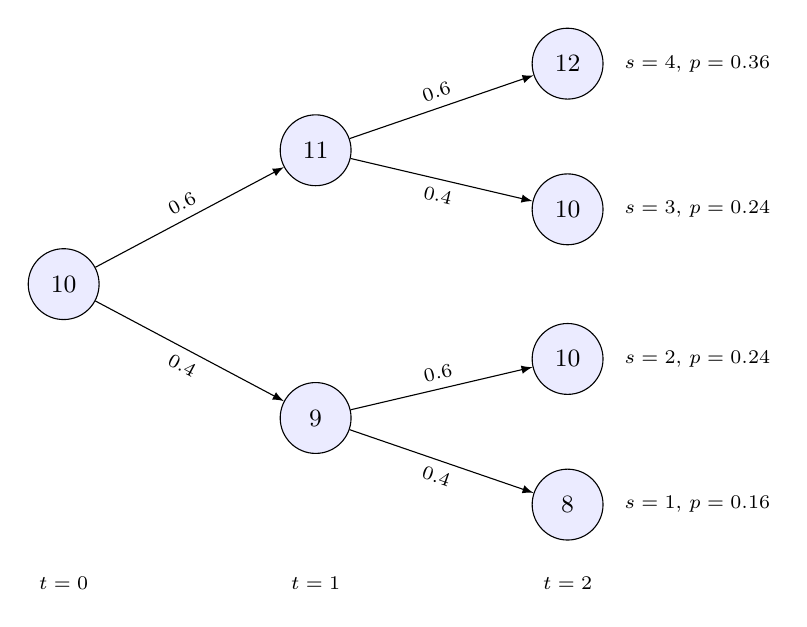
\begin{tikzpicture}[x=1cm,y=1cm,>=latex,font=\small,
  nd/.style={draw,circle,inner sep=1.4pt,minimum size=9mm,fill=blue!8},
  lb/.style={font=\scriptsize,midway,sloped,above}]
  \node[nd] (r)  at (0,0)      {$10$};
  \node[nd] (u)  at (3.2,1.7)  {$11$};
  \node[nd] (d)  at (3.2,-1.7) {$9$};
  \node[nd] (uu) at (6.4,2.8)  {$12$};
  \node[nd] (ud) at (6.4,0.95) {$10$};
  \node[nd] (du) at (6.4,-0.95){$10$};
  \node[nd] (dd) at (6.4,-2.8) {$8$};
  \draw[->] (r)  -- node[lb]{$0.6$} (u);
  \draw[->] (r)  -- node[lb,below]{$0.4$} (d);
  \draw[->] (u)  -- node[lb]{$0.6$} (uu);
  \draw[->] (u)  -- node[lb,below]{$0.4$} (ud);
  \draw[->] (d)  -- node[lb]{$0.6$} (du);
  \draw[->] (d)  -- node[lb,below]{$0.4$} (dd);
  \node[right,font=\scriptsize] at (7.0,2.8)  {$s = 4$, $p = 0.36$};
  \node[right,font=\scriptsize] at (7.0,0.95) {$s = 3$, $p = 0.24$};
  \node[right,font=\scriptsize] at (7.0,-0.95){$s = 2$, $p = 0.24$};
  \node[right,font=\scriptsize] at (7.0,-2.8) {$s = 1$, $p = 0.16$};
  \node[font=\scriptsize,below] at (0,-3.6)   {$t = 0$};
  \node[font=\scriptsize,below] at (3.2,-3.6) {$t = 1$};
  \node[font=\scriptsize,below] at (6.4,-3.6) {$t = 2$};
\end{tikzpicture}
\end{center}

\textbf{(b)(i) Extensive form.} Attach one decision to each \emph{node} of the
tree: $x_0$ at the root, $x_{1,1}$, $x_{1,2}$ at stage 1, and
$x_{2,1}, \ldots, x_{2,4}$ at stage 2, with the states $s$ indexed likewise.
Writing the cost of a node times the probability of reaching it,
\begin{align*}
\min\ & 10x_0
 + 0.4\left(9x_{1,1} + 0.4 \cdot 8 x_{2,1} + 0.6 \cdot 10 x_{2,2}\right)
 + 0.6\left(11x_{1,2} + 0.4 \cdot 10 x_{2,3} + 0.6 \cdot 12 x_{2,4}\right) \\
\text{s.t. } & s_0 = x_0, \\
& s_{1,1} = s_0 + x_{1,1}, \qquad s_{1,2} = s_0 + x_{1,2}, \\
& s_{2,1} = s_{1,1} + x_{2,1}, \quad s_{2,2} = s_{1,1} + x_{2,2}, \quad
  s_{2,3} = s_{1,2} + x_{2,3}, \quad s_{2,4} = s_{1,2} + x_{2,4}, \\
& s_{2,j} = a, \quad j = 1,\ldots,4, \\
& x \geq 0, \quad s \geq 0,
\end{align*}
where node $(1,1)$ carries $\xi_1 = 9$ and node $(1,2)$ carries $\xi_1 = 11$.

\textbf{(b)(ii) Scenario decomposition.} Attach instead one full decision path to
each \emph{scenario}: $x_t^{(s)}$ and $s_t^{(s)}$, $t = 0,1,2$, $s = 1,\ldots,4$.
With $p = (0.16, 0.24, 0.24, 0.36)$ and the cost paths $(10,9,8)$, $(10,9,10)$,
$(10,11,10)$, $(10,11,12)$,
\begin{align*}
\min\ & 0.16\left(10x_0^{(1)} + 9x_1^{(1)} + 8x_2^{(1)}\right)
      + 0.24\left(10x_0^{(2)} + 9x_1^{(2)} + 10x_2^{(2)}\right) \\
& + 0.24\left(10x_0^{(3)} + 11x_1^{(3)} + 10x_2^{(3)}\right)
  + 0.36\left(10x_0^{(4)} + 11x_1^{(4)} + 12x_2^{(4)}\right) \\
\text{s.t. } & s_0^{(s)} = x_0^{(s)}, \quad
 s_t^{(s)} = s_{t-1}^{(s)} + x_t^{(s)}, \quad t = 1,2, \quad s = 1,\ldots,4, \\
& s_2^{(s)} = a, \quad x_t^{(s)} \geq 0, \quad s_t^{(s)} \geq 0, \\
& x_0^{(1)} = x_0^{(2)} = x_0^{(3)} = x_0^{(4)}, & \text{(non-anticipativity, $t=0$)} \\
& x_1^{(1)} = x_1^{(2)}, \qquad x_1^{(3)} = x_1^{(4)}. & \text{(non-anticipativity, $t=1$)}
\end{align*}

\textbf{(c)} Only in the scenario decomposition. The extensive form attaches one
variable per \emph{node}, so two scenarios that are indistinguishable at time $t$
automatically share the same decision: non-anticipativity is built into the
indexing. The scenario decomposition duplicates the decisions along each path,
which is what makes the problem separable by scenario, and the coupling must
then be restored explicitly. Those are precisely the constraints that deck~08
dualizes, with multipliers $\pi$, and that progressive hedging enforces
iteratively.

Note the pattern: at $t = 2$ the four scenarios are all distinguishable, so no
constraint is needed; at $t = 1$ they form two groups; at $t = 0$ a single one.
\end{solution}

%%%%%%%%%%%%%%%%%%%%%%%%%%%%%%%%%%%%%%%%%%%%%%%%%%%%%%%%%%%%%%%%%%%%%%%%%%%%%%
\section{Monte Carlo approximation}
%%%%%%%%%%%%%%%%%%%%%%%%%%%%%%%%%%%%%%%%%%%%%%%%%%%%%%%%%%%%%%%%%%%%%%%%%%%%%%

\begin{exercise}
(Decks~03 and~09.) Show that
\[
\EE_{\bsxi}\left[ \min_{x \in \calX} z(x,\bsxi) \right] \leq \min_{x \in \calX} \EE_{\bsxi}\left[ z(x,\bsxi) \right]
\]
for a deterministic feasible set $\calX$. How is this result to be interpreted
for stochastic programming? Extend it to a Monte Carlo sample average.
\end{exercise}

\begin{solution}
Assume the expectations are well defined and the minima attained, as the
statement implicitly does. There exists $x^* \in \calX$ with
$\min_{x \in \calX} \EE_{\bsxi}[z(x,\bsxi)] = \EE_{\bsxi}[z(x^*,\bsxi)]$. Since
$x^* \in \calX$,
\[
\min_{x \in \calX} z(x,\xi) \leq z(x^*,\xi) \quad \text{for every } \xi,
\]
and taking expectations gives the result.

Without attainment the statement still holds with infima: for every
$y \in \calX$, $\inf_{x \in \calX} z(x,\bsxi) \leq z(y,\bsxi)$, hence
$\EE_{\bsxi}[\inf_{x \in \calX} z(x,\bsxi)] \leq \EE_{\bsxi}[z(y,\bsxi)]$, and
taking the infimum over $y$ closes the argument.

\textbf{Interpretation.} This is $\WSv \leq \RPv$ of deck~03: minimizing under
perfect information is optimistic. A decision tailored to each realization can
only beat a single decision that must serve them all.

\textbf{Extension to sampling.} Let
$z_N(x) = \frac{1}{N}\sum_{n=1}^N z(x,\bsxi_n)$ be the sample average over an
i.i.d.\ sample. The result just proved applies verbatim with the random element
taken to be the whole sample $(\bsxi_1,\ldots,\bsxi_N)$ and the function
$z_N$ in place of $z$:
\[
\EE\left[ \min_{x \in \calX} z_N(x) \right]
\ \leq\ \min_{x \in \calX} \EE\left[ z_N(x) \right]
\ =\ \min_{x \in \calX} \EE_{\bsxi}\left[ z(x,\bsxi) \right],
\]
the last equality because $z_N(x)$ is an unbiased estimator of
$\EE_{\bsxi}[z(x,\bsxi)]$ for each fixed $x$.

\medskip
\emph{Caution.} One cannot argue by exchanging the minimum and the sum, writing
$\min_x \frac{1}{N}\sum_n z(x,\bsxi_n) = \frac{1}{N}\sum_n \min_x z(x,\bsxi_n)$:
the minimum of a sum is not the sum of the minima, and the inequality in fact
runs the other way,
\[
\min_{x \in \calX} \frac{1}{N}\sum_{n=1}^N z(x,\bsxi_n)
\ \geq\ \frac{1}{N}\sum_{n=1}^N \min_{x \in \calX} z(x,\bsxi_n),
\]
since a single $x$ must serve all $N$ draws. That route does not close the chain;
the one above does.

\medskip
The conclusion is that the sample-average optimal value is a
\emph{downward-biased} estimator of the true optimal value: the optimizer
exploits the particular sample it was given. This is the bias that deck~09
analyses, and why an out-of-sample evaluation is needed to obtain an honest upper
bound.
\end{solution}

\end{document}
"
% The Makefile target `exercises` builds both. Nothing has to be kept in sync.
\newif\ifsolutions
\solutionstrue
\ifdefined\nosolutions\solutionsfalse\fi

\newcounter{exercisecount}[section]
\renewcommand{\theexercisecount}{\thesection.\arabic{exercisecount}}
\newenvironment{exercise}
  {\par\medskip\refstepcounter{exercisecount}%
   \noindent\textbf{Exercise \theexercisecount.}\begin{itshape}}
  {\end{itshape}\par\medskip}

\ifsolutions
  \newenvironment{solution}
    {\par\nobreak\smallskip\noindent\textbf{Solution.}\par\nobreak\smallskip}
    {\par\medskip\hrule height 0pt\medskip}
\else
  \excludecomment{solution}
\fi

\newcommand{\WSv}{\mathrm{WS}}
\newcommand{\RPv}{\mathrm{RP}}
\newcommand{\EVv}{\mathrm{EV}}
\newcommand{\EEVv}{\mathrm{EEV}}
\newcommand{\EVPIv}{\mathrm{EVPI}}
\newcommand{\VSSv}{\mathrm{VSS}}

\title{Stochastic optimization\\[2mm] \Large Exercise collection%
\ifsolutions\\[2mm]\normalsize with solutions\fi}
\author{Fabian Bastin\\ \small Université de Montréal -- CIRRELT -- IVADO}
\date{}

\begin{document}

\maketitle

\noindent
This collection accompanies the lecture slides. Each exercise names the deck it
depends on.
\ifsolutions
This is the version \emph{with solutions}; the statements alone are in
\texttt{exercises.pdf}.
\else
This version holds the \emph{statements only}; the solutions are in
\texttt{exercises\_solutions.pdf}.
\fi

\medskip
\noindent
Sources are indicated exercise by exercise; several are adapted from Birge and
Louveaux, \emph{Introduction to Stochastic Programming}, 2nd edition, Springer,
2011.

\tableofcontents

%%%%%%%%%%%%%%%%%%%%%%%%%%%%%%%%%%%%%%%%%%%%%%%%%%%%%%%%%%%%%%%%%%%%%%%%%%%%%%
\section{Generalities}
%%%%%%%%%%%%%%%%%%%%%%%%%%%%%%%%%%%%%%%%%%%%%%%%%%%%%%%%%%%%%%%%%%%%%%%%%%%%%%

\begin{exercise}
(Deck~03.) Show that the value of the stochastic solution and the expected value
of perfect information are always non-negative.
\end{exercise}

\begin{solution}
Consider the general problem $\min_{x \in X} \EE[z(x,\bsxi)]$, and recall the
four quantities
\[
\RPv = \min_{x \in X} \EE[z(x,\bsxi)], \qquad
\WSv = \EE\left[ \min_{x \in X} z(x,\bsxi) \right], \qquad
\EVv = \min_{x \in X} z(x, \overline{\xi}), \quad \overline{\xi} = \EE[\bsxi],
\]
and
\[
\EEVv = \EE\left[ z\!\left(\overline{x}(\overline{\xi}), \bsxi\right) \right],
\qquad \overline{x}(\overline{\xi}) \in \arg\min_{x \in X} z(x,\overline{\xi}).
\]

\emph{A warning on $\EEVv$.} It is \textbf{not} $\EE[\EVv]$: $\EVv$ is a
deterministic number, so $\EE[\EVv] = \EVv$. $\EEVv$ is the expected cost of
\emph{using} the expected-value decision, the uncertainty being restored
afterwards. This is exactly what makes $\VSSv$ measure something.

\medskip
$\VSSv = \EEVv - \RPv \geq 0$. Since $\overline{x}(\overline{\xi}) \in X$, it is
one particular feasible point of the recourse problem, so
\[
\RPv = \min_{x \in X} \EE[z(x,\bsxi)] \leq \EE\left[z\!\left(\overline{x}(\overline{\xi}),\bsxi\right)\right] = \EEVv .
\]

\medskip
$\EVPIv = \RPv - \WSv \geq 0$. Let $x^*_{\RPv} \in \arg\min_{x \in X} \EE[z(x,\bsxi)]$.
For every realization $\xi$,
\[
z(x^*_{\RPv}, \xi) \geq \min_{x \in X} z(x,\xi),
\]
and taking expectations, which preserves inequalities,
\[
\RPv = \EE\left[z(x^*_{\RPv},\bsxi)\right] \geq \EE\left[\min_{x \in X} z(x,\bsxi)\right] = \WSv .
\]

\medskip
Both arguments have the same shape: a single decision that must serve every
realization can only be worse than a decision tailored to each one.
\end{solution}

%%%%%%%%%%%%%%%%%%%%%%%%%%%%%%%%%%%%%%%%%%%%%%%%%%%%%%%%%%%%%%%%%%%%%%%%%%%%%%
\section{Two-stage problems with recourse}
%%%%%%%%%%%%%%%%%%%%%%%%%%%%%%%%%%%%%%%%%%%%%%%%%%%%%%%%%%%%%%%%%%%%%%%%%%%%%%

\begin{exercise}
(Deck~01 and~03.) Consider the farmer problem of deck~01. Is its recourse
\emph{complete}? \emph{Relatively complete}? \emph{Simple}?
\end{exercise}

\begin{solution}
Write $t_1$, $t_2$, $t_3$ for the yields (tons per acre) of one scenario, $y_1$,
$y_2$ for the tons of wheat and corn bought, $w_1$, $w_2$ for the tons sold, and
$w_3$, $w_4$ for the tons of sugar beets sold at the high and at the low price.
Given the acreages $x$, the second stage is
\begin{align*}
\min_{y,w}\ & 238y_1 - 170w_1 + 210y_2 - 150w_2 - 36w_3 - 10w_4 \\
\text{s.t. } & t_1x_1 + y_1 - w_1 \geq 200, \qquad t_2x_2 + y_2 - w_2 \geq 240, \\
& w_3 + w_4 \leq t_3x_3, \qquad w_3 \leq 6000, \qquad y, w \geq 0.
\end{align*}
Adding slacks $s \geq 0$ and moving $x$ to the right-hand side,
\[
y_1 - w_1 - s_1 = 200 - t_1x_1, \quad
y_2 - w_2 - s_2 = 240 - t_2x_2, \quad
w_3 + w_4 + s_3 = t_3x_3, \quad
w_3 + s_4 = 6000,
\]
so that, with the columns ordered as $(y_1, y_2, w_1, w_2, w_3, w_4, s_1, s_2, s_3, s_4)$,
\[
W = \begin{pmatrix}
1 & 0 & -1 & 0 & 0 & 0 & -1 & 0 & 0 & 0 \\
0 & 1 & 0 & -1 & 0 & 0 & 0 & -1 & 0 & 0 \\
0 & 0 & 0 & 0 & 1 & 1 & 0 & 0 & 1 & 0 \\
0 & 0 & 0 & 0 & 1 & 0 & 0 & 0 & 0 & 1
\end{pmatrix}.
\]

\textbf{Not complete.} Rows 3 and 4 meet only columns with non-negative entries,
so every $z \in \operatorname{pos} W$ has $z_3 \geq 0$ and $z_4 \geq 0$.
Conversely any such $z$ is attained (take $w_3 = 0$, $s_4 = z_4$, $w_4 = z_3$,
$s_3 = 0$, and use $(y_1,w_1)$, $(y_2,w_2)$ for the first two rows, which are
unrestricted). Hence
$\operatorname{pos} W = \RR \times \RR \times \RR_+ \times \RR_+ \neq \RR^4$.

\textbf{Relatively complete.} We need $h(\xi) - T(\xi)x \in \operatorname{pos} W$
for every $x \in K_1 = \lbrace x \in \RR^3_+ \mid x_1+x_2+x_3 \leq 500 \rbrace$
and every scenario. Its third and fourth components are $t_3x_3$ and $6000$,
both non-negative since $x_3 \geq 0$ and the yields are positive. So
$K_1 \subseteq K_2$. Concretely, buying all the wheat and corn needed and selling
no sugar beets is feasible whatever the seeding decision and the yields ---
expensive, but feasible.

\textbf{Not simple.} Simple recourse requires $W = \begin{pmatrix} I & -I \end{pmatrix}$.
Here $W$ is $4 \times 10$ and $w_3$ appears in two rows, the quota coupling the
beet sales to the harvest.

\medskip
Completeness is read off $W$ alone and fails here on a technicality; relative
completeness --- the property that matters --- holds because every right-hand
side the model can produce lands in $\operatorname{pos} W$.
\end{solution}

\begin{exercise}
(Deck~03; Birge and Louveaux, p.~87.) Consider the second-stage program
\[
Q(x,\xi) = \min_y \lbrace y \mid \xi y = 1-x,\ y \geq 0 \rbrace,
\]
where $\bsxi$ follows a triangular distribution on $[0,1]$, i.e.\ $P[\bsxi \leq u] = u^2$.
\begin{enumerate}[(a)]
\item Is the recourse fixed? Why?
\item Express $K_2(\xi)$ for every $\xi \in [0,1]$.
\item Express $K_2$, $K_2^P$ and $\calQ$.
\end{enumerate}
\end{exercise}

\begin{solution}
\textbf{(a)} The recourse is \emph{not} fixed: here $W \equiv \bsxi$, which is
random. Moreover $\xi$ can take the value $0$, so the transformation
$y = (1-x)/\xi$ is not defined on all of $\Xi = [0,1]$. In terms of the cone,
\[
\operatorname{pos} W =
\begin{cases}
\lbrace 0 \rbrace & \text{if } \xi = 0, \\
\RR_+ & \text{if } \xi \neq 0.
\end{cases}
\]

\textbf{(b)} Two cases.
\emph{$\xi \in (0,1]$:} since $y \geq 0$ and $\xi > 0$, feasibility requires
$1-x \geq 0$, so $K_2(\xi) = \lbrace x \mid x \leq 1 \rbrace$, with
$Q(x,\xi) = (1-x)/\xi$ attained at $y^* = (1-x)/\xi$.
\emph{$\xi = 0$:} no $y$ satisfies $0 \cdot y = 1-x$ unless $x = 1$, so
$K_2(0) = \lbrace 1 \rbrace$.

\textbf{(c)} Therefore
\[
K_2^P = \lbrace x \mid x \leq 1 \rbrace \cap \lbrace 1 \rbrace = \lbrace 1 \rbrace,
\]
while, since $P[\bsxi = 0] = 0$ and the density is $f(\xi) = 2\xi$,
\[
\calQ(x) = \int_0^1 \frac{1-x}{\xi}\, 2\xi \, d\xi = 2(1-x), \qquad \forall x \leq 1,
\]
so $K_2 = \lbrace x \mid x \leq 1 \rbrace$ and $K_2^P \subsetneq K_2$.

\medskip
The difference is that a point leaves $K_2^P$ as soon as it is infeasible for
\emph{one} value of $\xi$, whatever its probability, whereas $K_2$ ignores
infeasibilities occurring with probability zero. Recall that for a program with
a \emph{fixed} recourse --- not the case here --- and $\bsxi$ with finite
second-order moments, we would have had $K_2 = K_2^P$.
\end{solution}

\begin{exercise}
(Deck~03.) Consider the second-stage program
\begin{align*}
\min_y\ & 2y_1+y_2\\
\text{s.t. } & y_1 - y_2 \leq 2-\bsxi x_1,\\
& y_2 \leq x_2,\\
& y_1, y_2 \geq 0.
\end{align*}
Find $K_2(\xi)$ and $K_2$ when (a) $\bsxi \sim U[0,1]$; (b) $\bsxi \sim \text{Poisson}(\lambda)$, $\lambda > 0$.
Which properties do you expect of $K_2$? Is the recourse simple or complete? If
not, under which conditions would it be relatively complete?
\end{exercise}

\begin{solution}
\textbf{The elementary set.} $y_2 \geq 0$ and $y_2 \leq x_2$ force $x_2 \geq 0$.
The first constraint then reads $y_1 \leq 2 - \xi x_1 + y_2$, and the largest
admissible right-hand side is obtained at $y_2 = x_2$; a feasible $y_1 \geq 0$
exists if and only if $2 - \xi x_1 + x_2 \geq 0$. Hence
\[
K_2(\xi) = \lbrace x \mid x_2 \geq 0,\ \xi x_1 \leq 2+x_2 \rbrace
= \lbrace x \mid x_2 \geq \max(0, \xi x_1 - 2) \rbrace .
\]

\textbf{(a) $\bsxi \sim U[0,1]$}, $\Xi = [0,1]$. The recourse is fixed ($\bsxi$
enters only through $T(\bsxi)$) and the distribution has finite second-order
moments, so $K_2 = K_2^s = K_2^P = \bigcap_{\xi \in \Xi} K_2(\xi)$.
For $x_1 \geq 0$ and $\xi \leq 1$, $\xi x_1 \leq x_1$, so
$x \in K_2(1) \Rightarrow x \in K_2(\xi)$; for $x_1 < 0$, $\xi x_1 \leq 0 \leq 2+x_2$
always. In both cases $K_2(1) \subseteq K_2(\xi)$ for every $\xi \in \Xi$: the
intersection is reached at $\xi = 1$ and
\[
K_2 = \lbrace x \mid x_2 \geq 0,\ x_1 \leq 2+x_2 \rbrace .
\]

\textbf{(b) $\bsxi \sim \text{Poisson}(\lambda)$}, $\Xi = \lbrace 0,1,2,\ldots\rbrace$
unbounded. If $x_1 > 0$ then $\xi x_1$ is unbounded above and no $x_2$ absorbs
it; if $x_1 \leq 0$ then $\xi x_1 \leq 0 \leq 2+x_2$. Hence
$K_2 = \lbrace x \mid x_1 \leq 0,\ x_2 \geq 0 \rbrace$.

\textbf{Expected properties.} Each $K_2(\xi)$ is an intersection of two
half-spaces, hence closed and convex, and so is $K_2$. This is no accident: with
a fixed recourse $x \in K_2(\xi) \iff h(\xi)-T(\xi)x \in \operatorname{pos} W$,
and $\operatorname{pos} W$ is a closed convex cone. With a finite support $K_2$
would moreover be polyhedral; here $\Xi$ is infinite, yet both answers happen to
be polyhedral.

\textbf{Type of recourse.} Putting the program in standard form with surplus
variables $s_1, s_2 \geq 0$,
\[
y_1 - y_2 + s_1 = 2 - \xi x_1, \qquad y_2 + s_2 = x_2,
\qquad
W = \begin{pmatrix} 1 & -1 & 1 & 0 \\ 0 & 1 & 0 & 1 \end{pmatrix}.
\]
The recourse is \emph{not simple} ($W$ is not $\begin{pmatrix} I & -I\end{pmatrix}$),
and \emph{not complete}: the second row involves only non-negative coefficients,
so $z_2 < 0$ is unreachable and $\operatorname{pos} W = \RR \times \RR_+ \neq \RR^2$.
It is \emph{relatively complete} exactly when $K_1 \subseteq K_2$, i.e.\ when the
first stage already enforces $x_2 \geq 0$ together with $x_1 \leq 2+x_2$ in
case~(a), or $x_1 \leq 0$ in case~(b). If the first stage merely requires
$x \geq 0$, then
\[
\text{(a)}\quad K_1 \cap K_2 \subseteq \lbrace x \geq 0 \mid x_1 \leq 2+x_2 \rbrace,
\qquad
\text{(b)}\quad K_1 \cap K_2 \subseteq \lbrace x \mid x_1 = 0,\ x_2 \geq 0 \rbrace .
\]
Relative completeness is plausible in the first case and very restrictive in the
second: an unbounded support is far less forgiving, since \emph{every}
realization has to be survived.
\end{solution}

\begin{exercise}
(Deck~03; Birge and Louveaux, p.~102.) Consider the second-stage program
\begin{align*}
\min_y\ & 2y_1+y_2\\
\text{s.t. } & y_1 + y_2 \geq 1-x_1,\\
& y_1 \geq \bsxi - x_1-x_2,\\
& y_1, y_2 \geq 0.
\end{align*}
Show that this program has a complete recourse when $\bsxi$ has a finite expectation.
\end{exercise}

\begin{solution}
\textbf{A direct argument.} Completeness asks that for every right-hand side
$(z_1, z_2)$ there exist $y_1, y_2 \geq 0$ with $y_1 + y_2 \geq z_1$ and
$y_1 \geq z_2$. Taking $y_1 = \max\lbrace 0, z_2 \rbrace$ satisfies the second,
and $y_2 = \max\lbrace 0, z_1 - y_1 \rbrace$ the first; both are non-negative.

\textbf{Through $\operatorname{pos} W$.} The standard characterisation requires
$Wy = z$ with $y \geq 0$, and is stated for equalities: showing that $Wy \geq z$
is solvable is \emph{not} the same statement. So bring the program to the
standard form first, with surplus variables $s \geq 0$:
\[
y_1 + y_2 - s_1 = 1-x_1, \qquad y_1 - s_2 = \xi - x_1 - x_2,
\qquad
W = \begin{pmatrix} 1 & 1 & -1 & 0 \\ 1 & 0 & 0 & -1 \end{pmatrix}.
\]
The second row leaves $y_1$ free to absorb the sign of $z_2$:
\[
\begin{cases}
y_1 = z_2,\ s_2 = 0 & \text{if } z_2 \geq 0,\\
y_1 = 0,\ s_2 = -z_2 & \text{otherwise.}
\end{cases}
\]
The first row then reads $y_2 - s_1 = z_1 - y_1$. If $z_2 \geq 0$, then
$y_2 - s_1 = z_1 - z_2$ and we take
\[
\begin{cases}
y_2 = z_1-z_2,\ s_1 = 0 & \text{if } z_1-z_2 \geq 0,\\
y_2 = 0,\ s_1 = z_2-z_1 & \text{otherwise;}
\end{cases}
\]
if $z_2 < 0$, then $y_1 = 0$, $y_2 - s_1 = z_1$, and it suffices to choose
\[
\begin{cases}
y_2 = z_1,\ s_1 = 0 & \text{if } z_1 \geq 0,\\
y_2 = 0,\ s_1 = -z_1 & \text{otherwise.}
\end{cases}
\]
Every $z \in \RR^2$ is reached, so $\operatorname{pos} W = \RR^2$ and the
recourse is complete.

\textbf{The hypothesis on $\EE[\bsxi]$ played no role}, and could not have:
completeness involves only $W$, which is fixed. The statement is copied from
Birge and Louveaux, where the hypothesis is superfluous at this point. In
particular it is \emph{not} what gives $K_2 = \RR^2$ --- completeness alone does.

What a finite expectation buys is the \emph{finiteness} of the recourse. Deck~03
uses exactly this $W$ with $P[\bsxi = 2^n] = 2^{-(n+1)}$, $n = 0,1,2,\ldots$, for
which $\EE[\bsxi] = +\infty$, to exhibit a problem where the recourse is complete
--- hence $K_2 = \RR^2$ --- while $\calQ(x) = +\infty$ everywhere, so
$K_2^s = \emptyset$. Complete recourse and finite recourse are two different
things.
\end{solution}

\begin{exercise}
(Deck~03.) A company must order a quantity $x$ of a product to meet a demand $d$
that is unknown at the time of ordering. The unit ordering cost is $c > 0$. If
$d > x$, a penalty $b \geq 0$ is incurred per unit of unmet demand; if $d < x$,
a holding cost $h$ is incurred per surplus unit.
\begin{enumerate}[(a)]
\item Formulate the problem as a two-stage stochastic program.
\item Is the recourse simple, complete, relatively complete?
\item What can be expected of the first-stage solution when $b < c$?
\end{enumerate}
\end{exercise}

\begin{solution}
\textbf{(a)} The first stage is the order; the second stage settles the
discrepancy between $x$ and the realized demand:
\[
\min_{x \geq 0}\ cx + \EE_{\bsd}[Q(x,\bsd)],
\qquad
Q(x,d) = \min_{y^+,y^- \geq 0} \lbrace by^+ + hy^- \mid y^+ - y^- = d-x \rbrace .
\]

\textbf{(b)} Here $W = \begin{pmatrix} 1 & -1 \end{pmatrix}$, so the recourse is
\emph{simple}, hence also complete and relatively complete. The finiteness
condition of the simple-recourse theorem reads $b + h \geq 0$, satisfied as soon
as both costs are non-negative.

\textbf{(c)} With $b < c$, an extra ordered unit costs more than the penalty it
avoids. Formally, the objective $cx + \EE[b(\bsd-x)^+ + h(x-\bsd)^+]$ has
right derivative at $x$ equal to $c - b\,P[\bsd > x] + h\,P[\bsd < x] \geq c - b > 0$,
so the objective is strictly increasing and $x^* = 0$: the company orders
nothing and pays the penalty.
\end{solution}

\begin{exercise}
(Deck~03.) A good $X$ must be produced before its demand is known. Each unit
produced costs \$2. Demand is discrete, taking the values $D_s$ with
probabilities $p_s$, $s = 1,\ldots,S$. Demand can also be met by buying from an
external supplier at \$3 per unit, once it has been observed. How much should be
produced now? Formulate the problem as a two-stage stochastic program minimizing
the expected production cost.
\end{exercise}

\begin{solution}
Let $x \geq 0$ be the number of units produced at the first stage, and
$y_s \geq 0$ the number bought from the external supplier in scenario $s$. Demand
is met when $x + y_s \geq D_s$, so
\begin{align*}
\min\ & 2x + \sum_{s=1}^S p_s\, 3 y_s \\
\text{s.t. } & x + y_s \geq D_s, \quad s = 1,\ldots,S, \\
& x \geq 0, \quad y_s \geq 0, \quad s = 1,\ldots,S.
\end{align*}
The second stage decomposes scenario by scenario, with $y_s = (D_s - x)^+$, so
the model is a simple-recourse one: producing is cheaper than outsourcing, but
must be committed to before the demand is known.
\end{solution}

\begin{exercise}
(Deck~03; Higle, \emph{Tutorials in Operations Research}, INFORMS, 2005.)
The Dakota Furniture Company makes desks, tables and chairs. Each item consumes
lumber and two kinds of skilled labour, finishing and carpentry:

\begin{center}
\begin{tabular}{|l|c|c|c|c|}
\hline
Resource & Cost & Desk & Table & Chair \\
\hline
Lumber (board ft.) & \$2 & 8 & 6 & 1 \\
Finishing (hours)  & \$4 & 4 & 2 & 1.5 \\
Carpentry (hours)  & \$5.2 & 2 & 1.5 & 0.5 \\
\hline
Selling price & & \$60 & \$40 & \$10 \\
\hline
\end{tabular}
\end{center}

Resources must be acquired before the demand is known. Three equally structured
demand scenarios are considered, with probabilities $0.3$, $0.4$ and $0.3$:

\begin{center}
\begin{tabular}{|l|c|c|c|}
\hline
Scenario & Desks & Tables & Chairs \\
\hline
Low ($p = 0.3$)         & 50  & 20  & 200 \\
Most likely ($p = 0.4$) & 150 & 110 & 225 \\
High ($p = 0.3$)        & 250 & 250 & 500 \\
\hline
\end{tabular}
\end{center}

Formulate the problem as a two-stage stochastic program maximizing the expected
profit. Only the formulation is asked.
\end{exercise}

\begin{solution}
Treat it as a resource-allocation problem. First stage: $x_1$ board feet of
lumber, $x_2$ finishing hours, $x_3$ carpentry hours. Second stage: $y_1$ desks,
$y_2$ tables, $y_3$ chairs produced once the demand is known.
\[
\min_{x \geq 0}\ 2x_1 + 4x_2 + 5.2x_3 + \EE_{\bsxi}[Q(x,\bsxi)],
\]
with
\begin{align*}
Q(x,\xi) = \min_y\ & -60y_1 - 40y_2 - 10y_3 \\
\text{s.t. } & 8y_1 + 6y_2 + y_3 \leq x_1, \\
& 4y_1 + 2y_2 + 1.5y_3 \leq x_2, \\
& 2y_1 + 1.5y_2 + 0.5y_3 \leq x_3, \\
& y_i \leq d_i(\xi),\ i = 1,2,3, \qquad y \geq 0 .
\end{align*}
Maximizing profit is minimizing its negative, hence the signs in $Q$. With the
three scenarios,
\[
\EE_{\bsxi}[Q(x,\bsxi)] = 0.3\,Q(x,\xi_1) + 0.4\,Q(x,\xi_2) + 0.3\,Q(x,\xi_3),
\]
where $d(\xi_1) = (50,20,200)$, $d(\xi_2) = (150,110,225)$ and
$d(\xi_3) = (250,250,500)$.
\end{solution}

\begin{exercise}
(Deck~03; Birge and Louveaux, p.~142.) Consider
\begin{align*}
\min_x\ & x_1 + 4x_2 + \EE_{\bsxi}[Q(x,\bsxi)] \\
\text{s.t. } & x_1 + x_2 = 1, \quad x \geq 0,
\end{align*}
with
\begin{align*}
Q(x,\xi) = \min_y\ & y_1 + 10y_2 + 10y_3 \\
\text{s.t. } & y_1 + y_2 - y_3 = \xi + x_1 - 2x_2, \\
& y_1 \leq 2, \qquad y \geq 0,
\end{align*}
and $\bsxi \sim U[1,3]$.
\begin{enumerate}[(a)]
\item Is the recourse fixed, simple, complete, relatively complete? Answer true
or false for each, with a brief justification.
\item For given $x$ and $\xi$, show, by discussing the value of $\xi + x_1 - 2x_2$, that
\[
y^*(x,\xi) =
\begin{cases}
y_1 = \xi + x_1 - 2x_2,\ y_2 = y_3 = 0 & \text{if } 0 \leq \xi + x_1 - 2x_2 \leq 2,\\
y_1 = 2,\ y_2 = \xi + x_1 - 2x_2 - 2,\ y_3 = 0 & \text{if } \xi + x_1 - 2x_2 > 2,\\
y_3 = 2x_2 - \xi - x_1,\ y_1 = y_2 = 0 & \text{if } \xi + x_1 - 2x_2 < 0.
\end{cases}
\]
\item Which expected property of $Q(x,\xi)$ does $y^*(x,\xi)$ confirm?
\item Is $\calQ(x) = \EE_{\bsxi}[Q(x,\bsxi)]$ differentiable? Why?
\item Express $K_1$, $K_2(\xi)$, $K_2^P$ and $K_2$.
\item Give the deterministic equivalent (extensive form) of the discretized
problem where $\bsxi$ takes the values $1$, $2$, $3$.
\end{enumerate}
\end{exercise}

\begin{solution}
\textbf{(a)} Adding a slack $y_4$ to the second constraint puts the second stage
in standard form,
\[
y_1 + y_2 - y_3 = \xi + x_1 - 2x_2, \qquad y_1 + y_4 = 2,
\qquad
W = \begin{pmatrix} 1 & 1 & -1 & 0 \\ 1 & 0 & 0 & 1 \end{pmatrix}.
\]
\emph{Fixed}: true, $W$ does not depend on $\xi$.
\emph{Simple}: false, $W$ is not of the form $\begin{pmatrix} I & -I\end{pmatrix}$.
\emph{Complete}: false --- the second row reads $y_1 + y_4 = z_2$ with
$y_1, y_4 \geq 0$, so no $z_2 < 0$ is reachable.
\emph{Relatively complete}: true. For any $x \in K_1$ and any $\xi$, the point
\[
y_1 = 0, \quad y_2 = (\xi + x_1 - 2x_2)^+, \quad y_3 = (-\xi - x_1 + 2x_2)^+, \quad y_4 = 2
\]
is feasible, the second component of the right-hand side being the constant $2 \geq 0$.

\textbf{(b)} Write $d = \xi + x_1 - 2x_2$. If $d < 0$, the only feasible extreme
point is $y_1 = y_2 = 0$, $y_3 = -d$, $y_4 = 2$, hence optimal. If $d \geq 0$,
an extreme point has $y_3 = 0$ and $y_1 + y_2 = d$ with $y_1 \leq 2$. Since the
cost of $y_1$ is $1$ and that of $y_2$ is $10$, $y_1$ is pushed as far as
possible: $y_1 = \min\lbrace d, 2 \rbrace$. This splits into $d \leq 2$, giving
$y_1 = d$, $y_2 = 0$, and $d \geq 2$, giving $y_1 = 2$, $y_2 = d-2$, as announced.

\textbf{(c)} $Q(\cdot,\xi)$ is convex and piecewise linear in the first-stage
decision $x$: the three regimes above are the three linear pieces, with
breakpoints where $d = 0$ and $d = 2$.

\textbf{(d)} Yes. $\bsxi$ is continuous with an absolutely continuous
distribution and finite second-order moments, so $\calQ$ is differentiable on the
interior of $K_2$: integrating over $\xi$ smooths away the kinks of each
$Q(\cdot,\xi)$.

\textbf{(e)} Directly from the statement,
$K_1 = \lbrace x \mid x_1 + x_2 = 1,\ x \geq 0 \rbrace$.
From (b), the second stage is feasible whatever $d$, so
$K_2(\xi) = \RR^2$ for every $\xi$, and therefore
$K_2^P = \bigcap_{\xi \in \Xi} K_2(\xi) = \RR^2$ and $K_2 = \RR^2$ as well.
In particular $K_1 \subseteq K_2$, confirming (a).

\textbf{(f)} With $\xi_1 = 1$, $\xi_2 = 2$, $\xi_3 = 3$ and $p_i = 1/3$,
\begin{align*}
\min\ & x_1 + 4x_2 + \sum_{i=1}^3 p_i\left(y_{1i} + 10y_{2i} + 10y_{3i}\right) \\
\text{s.t. } & x_1 + x_2 = 1, \\
& y_{1i} + y_{2i} - y_{3i} = \xi_i + x_1 - 2x_2, \quad i = 1,2,3, \\
& y_{1i} \leq 2, \quad i = 1,2,3, \\
& x \geq 0, \quad y_{1i}, y_{2i}, y_{3i} \geq 0, \quad i = 1,2,3.
\end{align*}
\end{solution}

%%%%%%%%%%%%%%%%%%%%%%%%%%%%%%%%%%%%%%%%%%%%%%%%%%%%%%%%%%%%%%%%%%%%%%%%%%%%%%
\section{Decomposition methods}
%%%%%%%%%%%%%%%%%%%%%%%%%%%%%%%%%%%%%%%%%%%%%%%%%%%%%%%%%%%%%%%%%%%%%%%%%%%%%%

\begin{exercise}
(Deck~04.) Consider
\begin{align*}
\min\ & 100x_1 + 150x_2 + \EE_{\bsxi}[q_1y_1 + q_2y_2] \\
\text{s.t. } & x_1 + x_2 \leq 120, \\
& 6y_1 + 10y_2 \leq 60x_1, \qquad 8y_1 + 5y_2 \leq 80x_2, \\
& y_1 \leq d_1, \qquad y_2 \leq d_2, \\
& x_1 \geq 40,\ x_2 \geq 20, \qquad y_1, y_2 \geq 0,
\end{align*}
under two scenarios $\bsxi = (d_1, d_2, q_1, q_2)$: $\xi_1 = (500, 100, -24, -28)$
with probability $p_1 = 0.4$, and $\xi_2 = (300, 300, -28, -32)$ with
probability $p_2 = 0.6$.

Run the first iteration of the single-cut $L$-shaped method, showing that the
second-stage solutions are respectively $y^* = (137.5, 100)$ and
$y^* = (80, 192)$. To obtain the dual solutions, use complementary slackness: a
dual variable can be non-zero only if the associated primal constraint is active.
\end{exercise}

\begin{solution}
\textbf{Master problem.} With no cut yet,
$\min \lbrace 100x_1 + 150x_2 \mid x_1 + x_2 \leq 120,\ x_1 \geq 40,\ x_2 \geq 20 \rbrace$,
whose optimal solution is immediately $x^1 = (40, 20)$, so $60x_1 = 2400$ and
$80x_2 = 1600$.

Since $x_1, x_2 \geq 0$ makes the second stage always feasible, the recourse is
relatively complete and no feasibility cut is needed.

\textbf{First scenario.}
$\min -24y_1 - 28y_2$ s.t. $6y_1 + 10y_2 \leq 2400$, $8y_1 + 5y_2 \leq 1600$,
$y_1 \leq 500$, $y_2 \leq 100$, $y \geq 0$.
We cannot have $y_1 = 500$, as the second constraint would be violated.
Setting $y_2 = 100$,
\[
y_1 = \min\left\lbrace \frac{2400-1000}{6},\ \frac{1600-500}{8} \right\rbrace
= \min\left\lbrace \frac{1400}{6},\ \frac{1100}{8} \right\rbrace
= \min\left\lbrace 233.33,\ 137.5 \right\rbrace = 137.5 .
\]
The alternative, making the first two constraints active, solves
$3y_1 + 5y_2 = 1200$ and $8y_1 + 5y_2 = 1600$, giving $y_1 = 80$, $y_2 = 192$,
which violates $y_2 \leq 100$. Hence $y^* = (137.5, 100)$, with objective
$-6100$.

Active constraints: the second and $y_2 \leq 100$. Complementary slackness gives
$\pi_1^* = \pi_3^* = 0$, and both $y_1, y_2 > 0$ make the dual constraints tight:
\[
8\pi_2^* = -24 \ \Rightarrow\ \pi_2^* = -3,
\qquad
5\pi_2^* + \pi_4^* = -28 \ \Rightarrow\ \pi_4^* = -28 + 15 = -13 .
\]

\textbf{Second scenario.}
$\min -28y_1 - 32y_2$, same first two constraints, $y_1 \leq 300$, $y_2 \leq 300$.
Taking $y_1 = 300$ or $y_2 = 300$ violates one of the first two constraints, so
both are active:
\[
3y_1 + 5y_2 = 1200, \qquad 8y_1 + 5y_2 = 1600
\ \Longrightarrow\ y^* = (80, 192),
\]
with objective $-8384$. Then $\pi_3^* = \pi_4^* = 0$ and
\[
6\pi_1^* + 8\pi_2^* = -28, \qquad 10\pi_1^* + 5\pi_2^* = -32 .
\]
Multiplying the first by $5$ and the second by $8$ and subtracting,
$50\pi_1^* = -116$, so $\pi_1^* = -2.32$; then
$5\pi_2^* = -32 + 23.2 = -8.8$, so $\pi_2^* = -1.76$.

\textbf{Optimality cut.} Writing the second-stage constraints as
$Wy \leq h(\xi) - T(\xi)x$,
\[
h(\xi_1) = \begin{pmatrix} 0 \\ 0 \\ 500 \\ 100 \end{pmatrix}, \quad
h(\xi_2) = \begin{pmatrix} 0 \\ 0 \\ 300 \\ 300 \end{pmatrix}, \quad
T(\xi_1) = T(\xi_2) = T = \begin{pmatrix} -60 & 0 \\ 0 & -80 \\ 0 & 0 \\ 0 & 0 \end{pmatrix}.
\]
Hence
\[
e_1 = 0.4\,\pi_1^{*T}h(\xi_1) + 0.6\,\pi_2^{*T}h(\xi_2)
= 0.4 \times (-1300) + 0.6 \times 0 = -520,
\]
and
\[
E_1 = 0.4\,\pi_1^{*T}T + 0.6\,\pi_2^{*T}T
= 0.4\begin{pmatrix} 0 & 240 \end{pmatrix} + 0.6\begin{pmatrix} 139.2 & 140.8 \end{pmatrix}
= \begin{pmatrix} 83.52 & 180.48 \end{pmatrix}.
\]
The cut $E_1x + \theta \geq e_1$ reads
\[
\theta \geq -520 - 83.52\,x_1 - 180.48\,x_2 ,
\]
and one checks that it is tight at $x^1 = (40,20)$:
$-520 - 3340.8 - 3609.6 = -7470.4 = 0.4(-6100) + 0.6(-8384) = \calQ(x^1)$,
as an optimality cut must be at the point where it was generated.

The master problem for the next iteration is therefore
\[
\min \lbrace 100x_1 + 150x_2 + \theta \mid x_1 + x_2 \leq 120,\ x_1 \geq 40,\ x_2 \geq 20,\
\theta \geq -520 - 83.52x_1 - 180.48x_2 \rbrace .
\]
\end{solution}

\begin{exercise}
(Deck~04.) In the regularized decomposition method of Ruszczy\'nski, what is the
difference between an \emph{exact} serious step and an \emph{approximate} serious
step? Why must the two be distinguished?
\end{exercise}

\begin{solution}
Briefly: the difference is whether the step can still be the optimal solution. In
both cases the incumbent moves because a better objective value has been found,
but after an approximate step we \emph{know} the solution is not optimal, whereas
after an exact step it might be.

In more detail, in the regularized method:
\begin{itemize}
\item
Step~4 is reached when \emph{no} optimality cut has been added. In the standard
$L$-shaped method this would already prove that the master solution is optimal,
but here the proximal penalty may have pulled the solution away from the true
minimizer, so the conclusion does not follow. The current first-stage point is
taken as the new incumbent and the method returns to step~1. The stopping test
there checks whether the master returns $x^{\nu} = a^{\nu}$: the penalty term
then vanishes, and since no new cut was produced, the solution is optimal.
Otherwise the penalty is what prevented optimality, and the method continues.
\item
Step~5 can only be reached when the condition of step~4 fails, i.e.\ when at
least one new optimality cut was added at step~3. A point at which a cut has just
been generated cannot be optimal --- the cut is violated there. It may still give
a better value of the full two-stage objective, in which case it is accepted as
the new incumbent, but we already know it is not the answer and must keep going.
\end{itemize}
\end{solution}

%%%%%%%%%%%%%%%%%%%%%%%%%%%%%%%%%%%%%%%%%%%%%%%%%%%%%%%%%%%%%%%%%%%%%%%%%%%%%%
\section{Multistage problems}
%%%%%%%%%%%%%%%%%%%%%%%%%%%%%%%%%%%%%%%%%%%%%%%%%%%%%%%%%%%%%%%%%%%%%%%%%%%%%%

\begin{exercise}
(Decks~06 and~08; Heitsch, Römisch and Strugarek, \emph{Stability of multistage
stochastic programs}, SIAM Journal on Optimization 17(2):511--525, 2006.)
Consider the stylized multistage program below, seeking an optimal purchasing
strategy under uncertain costs $\bsxi_t$ over the periods $t = 0,\ldots,T$. The
amounts purchased are $x_t$, and a prescribed amount $a$ must be reached at the
horizon $T$:
\begin{align*}
\min_{x}\ & \EE\left[ \sum_{t=0}^T \bsxi_t x_t \right], \\
\text{s.t. } & s_t - s_{t-1} = x_t, \quad t = 0,\ldots,T, \\
& s_{-1} = 0, \quad s_T = a, \quad x_t \geq 0, \quad s_t \geq 0,
\end{align*}
where $s_t$ is a state variable holding the amount accumulated at time $t$.

Take three stages ($t = 0, 1, 2$), a binary tree, and $\xi_0 = 10$; the cost goes
up by $1$ with probability $0.6$ and down by $1$ with probability $0.4$.
\begin{enumerate}[(a)]
\item Draw the scenario tree.
\item Write the problem (i) in extensive form, (ii) using a scenario decomposition.
\item In which of the two formulations must non-anticipativity constraints be
written explicitly?
\end{enumerate}
\end{exercise}

\begin{solution}
\textbf{(a)} Four scenarios, of probabilities $0.16$, $0.24$, $0.24$ and $0.36$:

\begin{center}
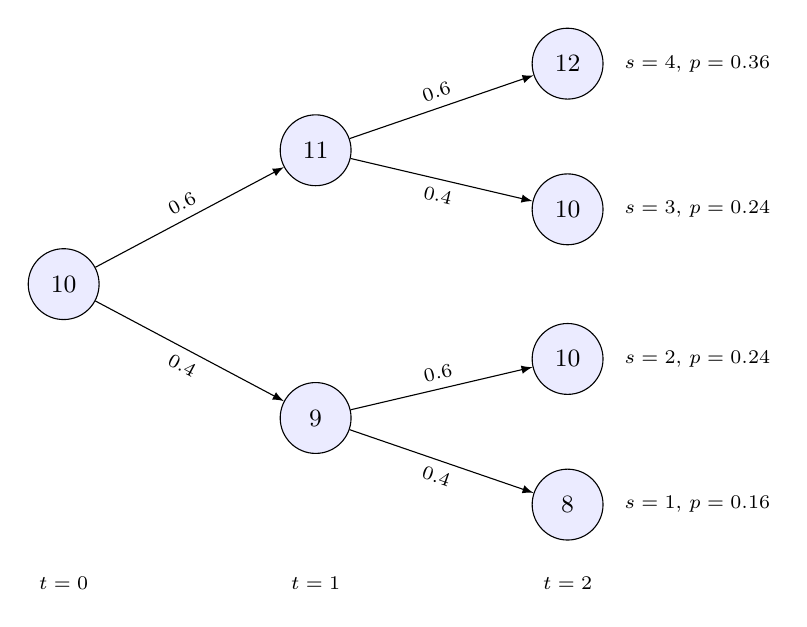
\begin{tikzpicture}[x=1cm,y=1cm,>=latex,font=\small,
  nd/.style={draw,circle,inner sep=1.4pt,minimum size=9mm,fill=blue!8},
  lb/.style={font=\scriptsize,midway,sloped,above}]
  \node[nd] (r)  at (0,0)      {$10$};
  \node[nd] (u)  at (3.2,1.7)  {$11$};
  \node[nd] (d)  at (3.2,-1.7) {$9$};
  \node[nd] (uu) at (6.4,2.8)  {$12$};
  \node[nd] (ud) at (6.4,0.95) {$10$};
  \node[nd] (du) at (6.4,-0.95){$10$};
  \node[nd] (dd) at (6.4,-2.8) {$8$};
  \draw[->] (r)  -- node[lb]{$0.6$} (u);
  \draw[->] (r)  -- node[lb,below]{$0.4$} (d);
  \draw[->] (u)  -- node[lb]{$0.6$} (uu);
  \draw[->] (u)  -- node[lb,below]{$0.4$} (ud);
  \draw[->] (d)  -- node[lb]{$0.6$} (du);
  \draw[->] (d)  -- node[lb,below]{$0.4$} (dd);
  \node[right,font=\scriptsize] at (7.0,2.8)  {$s = 4$, $p = 0.36$};
  \node[right,font=\scriptsize] at (7.0,0.95) {$s = 3$, $p = 0.24$};
  \node[right,font=\scriptsize] at (7.0,-0.95){$s = 2$, $p = 0.24$};
  \node[right,font=\scriptsize] at (7.0,-2.8) {$s = 1$, $p = 0.16$};
  \node[font=\scriptsize,below] at (0,-3.6)   {$t = 0$};
  \node[font=\scriptsize,below] at (3.2,-3.6) {$t = 1$};
  \node[font=\scriptsize,below] at (6.4,-3.6) {$t = 2$};
\end{tikzpicture}
\end{center}

\textbf{(b)(i) Extensive form.} Attach one decision to each \emph{node} of the
tree: $x_0$ at the root, $x_{1,1}$, $x_{1,2}$ at stage 1, and
$x_{2,1}, \ldots, x_{2,4}$ at stage 2, with the states $s$ indexed likewise.
Writing the cost of a node times the probability of reaching it,
\begin{align*}
\min\ & 10x_0
 + 0.4\left(9x_{1,1} + 0.4 \cdot 8 x_{2,1} + 0.6 \cdot 10 x_{2,2}\right)
 + 0.6\left(11x_{1,2} + 0.4 \cdot 10 x_{2,3} + 0.6 \cdot 12 x_{2,4}\right) \\
\text{s.t. } & s_0 = x_0, \\
& s_{1,1} = s_0 + x_{1,1}, \qquad s_{1,2} = s_0 + x_{1,2}, \\
& s_{2,1} = s_{1,1} + x_{2,1}, \quad s_{2,2} = s_{1,1} + x_{2,2}, \quad
  s_{2,3} = s_{1,2} + x_{2,3}, \quad s_{2,4} = s_{1,2} + x_{2,4}, \\
& s_{2,j} = a, \quad j = 1,\ldots,4, \\
& x \geq 0, \quad s \geq 0,
\end{align*}
where node $(1,1)$ carries $\xi_1 = 9$ and node $(1,2)$ carries $\xi_1 = 11$.

\textbf{(b)(ii) Scenario decomposition.} Attach instead one full decision path to
each \emph{scenario}: $x_t^{(s)}$ and $s_t^{(s)}$, $t = 0,1,2$, $s = 1,\ldots,4$.
With $p = (0.16, 0.24, 0.24, 0.36)$ and the cost paths $(10,9,8)$, $(10,9,10)$,
$(10,11,10)$, $(10,11,12)$,
\begin{align*}
\min\ & 0.16\left(10x_0^{(1)} + 9x_1^{(1)} + 8x_2^{(1)}\right)
      + 0.24\left(10x_0^{(2)} + 9x_1^{(2)} + 10x_2^{(2)}\right) \\
& + 0.24\left(10x_0^{(3)} + 11x_1^{(3)} + 10x_2^{(3)}\right)
  + 0.36\left(10x_0^{(4)} + 11x_1^{(4)} + 12x_2^{(4)}\right) \\
\text{s.t. } & s_0^{(s)} = x_0^{(s)}, \quad
 s_t^{(s)} = s_{t-1}^{(s)} + x_t^{(s)}, \quad t = 1,2, \quad s = 1,\ldots,4, \\
& s_2^{(s)} = a, \quad x_t^{(s)} \geq 0, \quad s_t^{(s)} \geq 0, \\
& x_0^{(1)} = x_0^{(2)} = x_0^{(3)} = x_0^{(4)}, & \text{(non-anticipativity, $t=0$)} \\
& x_1^{(1)} = x_1^{(2)}, \qquad x_1^{(3)} = x_1^{(4)}. & \text{(non-anticipativity, $t=1$)}
\end{align*}

\textbf{(c)} Only in the scenario decomposition. The extensive form attaches one
variable per \emph{node}, so two scenarios that are indistinguishable at time $t$
automatically share the same decision: non-anticipativity is built into the
indexing. The scenario decomposition duplicates the decisions along each path,
which is what makes the problem separable by scenario, and the coupling must
then be restored explicitly. Those are precisely the constraints that deck~08
dualizes, with multipliers $\pi$, and that progressive hedging enforces
iteratively.

Note the pattern: at $t = 2$ the four scenarios are all distinguishable, so no
constraint is needed; at $t = 1$ they form two groups; at $t = 0$ a single one.
\end{solution}

%%%%%%%%%%%%%%%%%%%%%%%%%%%%%%%%%%%%%%%%%%%%%%%%%%%%%%%%%%%%%%%%%%%%%%%%%%%%%%
\section{Monte Carlo approximation}
%%%%%%%%%%%%%%%%%%%%%%%%%%%%%%%%%%%%%%%%%%%%%%%%%%%%%%%%%%%%%%%%%%%%%%%%%%%%%%

\begin{exercise}
(Decks~03 and~09.) Show that
\[
\EE_{\bsxi}\left[ \min_{x \in \calX} z(x,\bsxi) \right] \leq \min_{x \in \calX} \EE_{\bsxi}\left[ z(x,\bsxi) \right]
\]
for a deterministic feasible set $\calX$. How is this result to be interpreted
for stochastic programming? Extend it to a Monte Carlo sample average.
\end{exercise}

\begin{solution}
Assume the expectations are well defined and the minima attained, as the
statement implicitly does. There exists $x^* \in \calX$ with
$\min_{x \in \calX} \EE_{\bsxi}[z(x,\bsxi)] = \EE_{\bsxi}[z(x^*,\bsxi)]$. Since
$x^* \in \calX$,
\[
\min_{x \in \calX} z(x,\xi) \leq z(x^*,\xi) \quad \text{for every } \xi,
\]
and taking expectations gives the result.

Without attainment the statement still holds with infima: for every
$y \in \calX$, $\inf_{x \in \calX} z(x,\bsxi) \leq z(y,\bsxi)$, hence
$\EE_{\bsxi}[\inf_{x \in \calX} z(x,\bsxi)] \leq \EE_{\bsxi}[z(y,\bsxi)]$, and
taking the infimum over $y$ closes the argument.

\textbf{Interpretation.} This is $\WSv \leq \RPv$ of deck~03: minimizing under
perfect information is optimistic. A decision tailored to each realization can
only beat a single decision that must serve them all.

\textbf{Extension to sampling.} Let
$z_N(x) = \frac{1}{N}\sum_{n=1}^N z(x,\bsxi_n)$ be the sample average over an
i.i.d.\ sample. The result just proved applies verbatim with the random element
taken to be the whole sample $(\bsxi_1,\ldots,\bsxi_N)$ and the function
$z_N$ in place of $z$:
\[
\EE\left[ \min_{x \in \calX} z_N(x) \right]
\ \leq\ \min_{x \in \calX} \EE\left[ z_N(x) \right]
\ =\ \min_{x \in \calX} \EE_{\bsxi}\left[ z(x,\bsxi) \right],
\]
the last equality because $z_N(x)$ is an unbiased estimator of
$\EE_{\bsxi}[z(x,\bsxi)]$ for each fixed $x$.

\medskip
\emph{Caution.} One cannot argue by exchanging the minimum and the sum, writing
$\min_x \frac{1}{N}\sum_n z(x,\bsxi_n) = \frac{1}{N}\sum_n \min_x z(x,\bsxi_n)$:
the minimum of a sum is not the sum of the minima, and the inequality in fact
runs the other way,
\[
\min_{x \in \calX} \frac{1}{N}\sum_{n=1}^N z(x,\bsxi_n)
\ \geq\ \frac{1}{N}\sum_{n=1}^N \min_{x \in \calX} z(x,\bsxi_n),
\]
since a single $x$ must serve all $N$ draws. That route does not close the chain;
the one above does.

\medskip
The conclusion is that the sample-average optimal value is a
\emph{downward-biased} estimator of the true optimal value: the optimizer
exploits the particular sample it was given. This is the bias that deck~09
analyses, and why an out-of-sample evaluation is needed to obtain an honest upper
bound.
\end{solution}

\end{document}
"
% The Makefile target `exercises` builds both. Nothing has to be kept in sync.
\newif\ifsolutions
\solutionstrue
\ifdefined\nosolutions\solutionsfalse\fi

\newcounter{exercisecount}[section]
\renewcommand{\theexercisecount}{\thesection.\arabic{exercisecount}}
\newenvironment{exercise}
  {\par\medskip\refstepcounter{exercisecount}%
   \noindent\textbf{Exercise \theexercisecount.}\begin{itshape}}
  {\end{itshape}\par\medskip}

\ifsolutions
  \newenvironment{solution}
    {\par\nobreak\smallskip\noindent\textbf{Solution.}\par\nobreak\smallskip}
    {\par\medskip\hrule height 0pt\medskip}
\else
  \excludecomment{solution}
\fi

\newcommand{\WSv}{\mathrm{WS}}
\newcommand{\RPv}{\mathrm{RP}}
\newcommand{\EVv}{\mathrm{EV}}
\newcommand{\EEVv}{\mathrm{EEV}}
\newcommand{\EVPIv}{\mathrm{EVPI}}
\newcommand{\VSSv}{\mathrm{VSS}}

\title{Stochastic optimization\\[2mm] \Large Exercise collection%
\ifsolutions\\[2mm]\normalsize with solutions\fi}
\author{Fabian Bastin\\ \small Université de Montréal -- CIRRELT -- IVADO}
\date{}

\begin{document}

\maketitle

\noindent
This collection accompanies the lecture slides. Each exercise names the deck it
depends on.
\ifsolutions
This is the version \emph{with solutions}; the statements alone are in
\texttt{exercises.pdf}.
\else
This version holds the \emph{statements only}; the solutions are in
\texttt{exercises\_solutions.pdf}.
\fi

\medskip
\noindent
Sources are indicated exercise by exercise; several are adapted from Birge and
Louveaux, \emph{Introduction to Stochastic Programming}, 2nd edition, Springer,
2011.

\tableofcontents

%%%%%%%%%%%%%%%%%%%%%%%%%%%%%%%%%%%%%%%%%%%%%%%%%%%%%%%%%%%%%%%%%%%%%%%%%%%%%%
\section{Generalities}
%%%%%%%%%%%%%%%%%%%%%%%%%%%%%%%%%%%%%%%%%%%%%%%%%%%%%%%%%%%%%%%%%%%%%%%%%%%%%%

\begin{exercise}
(Deck~03.) Show that the value of the stochastic solution and the expected value
of perfect information are always non-negative.
\end{exercise}

\begin{solution}
Consider the general problem $\min_{x \in X} \EE[z(x,\bsxi)]$, and recall the
four quantities
\[
\RPv = \min_{x \in X} \EE[z(x,\bsxi)], \qquad
\WSv = \EE\left[ \min_{x \in X} z(x,\bsxi) \right], \qquad
\EVv = \min_{x \in X} z(x, \overline{\xi}), \quad \overline{\xi} = \EE[\bsxi],
\]
and
\[
\EEVv = \EE\left[ z\!\left(\overline{x}(\overline{\xi}), \bsxi\right) \right],
\qquad \overline{x}(\overline{\xi}) \in \arg\min_{x \in X} z(x,\overline{\xi}).
\]

\emph{A warning on $\EEVv$.} It is \textbf{not} $\EE[\EVv]$: $\EVv$ is a
deterministic number, so $\EE[\EVv] = \EVv$. $\EEVv$ is the expected cost of
\emph{using} the expected-value decision, the uncertainty being restored
afterwards. This is exactly what makes $\VSSv$ measure something.

\medskip
$\VSSv = \EEVv - \RPv \geq 0$. Since $\overline{x}(\overline{\xi}) \in X$, it is
one particular feasible point of the recourse problem, so
\[
\RPv = \min_{x \in X} \EE[z(x,\bsxi)] \leq \EE\left[z\!\left(\overline{x}(\overline{\xi}),\bsxi\right)\right] = \EEVv .
\]

\medskip
$\EVPIv = \RPv - \WSv \geq 0$. Let $x^*_{\RPv} \in \arg\min_{x \in X} \EE[z(x,\bsxi)]$.
For every realization $\xi$,
\[
z(x^*_{\RPv}, \xi) \geq \min_{x \in X} z(x,\xi),
\]
and taking expectations, which preserves inequalities,
\[
\RPv = \EE\left[z(x^*_{\RPv},\bsxi)\right] \geq \EE\left[\min_{x \in X} z(x,\bsxi)\right] = \WSv .
\]

\medskip
Both arguments have the same shape: a single decision that must serve every
realization can only be worse than a decision tailored to each one.
\end{solution}

%%%%%%%%%%%%%%%%%%%%%%%%%%%%%%%%%%%%%%%%%%%%%%%%%%%%%%%%%%%%%%%%%%%%%%%%%%%%%%
\section{Two-stage problems with recourse}
%%%%%%%%%%%%%%%%%%%%%%%%%%%%%%%%%%%%%%%%%%%%%%%%%%%%%%%%%%%%%%%%%%%%%%%%%%%%%%

\begin{exercise}
(Deck~01 and~03.) Consider the farmer problem of deck~01. Is its recourse
\emph{complete}? \emph{Relatively complete}? \emph{Simple}?
\end{exercise}

\begin{solution}
Write $t_1$, $t_2$, $t_3$ for the yields (tons per acre) of one scenario, $y_1$,
$y_2$ for the tons of wheat and corn bought, $w_1$, $w_2$ for the tons sold, and
$w_3$, $w_4$ for the tons of sugar beets sold at the high and at the low price.
Given the acreages $x$, the second stage is
\begin{align*}
\min_{y,w}\ & 238y_1 - 170w_1 + 210y_2 - 150w_2 - 36w_3 - 10w_4 \\
\text{s.t. } & t_1x_1 + y_1 - w_1 \geq 200, \qquad t_2x_2 + y_2 - w_2 \geq 240, \\
& w_3 + w_4 \leq t_3x_3, \qquad w_3 \leq 6000, \qquad y, w \geq 0.
\end{align*}
Adding slacks $s \geq 0$ and moving $x$ to the right-hand side,
\[
y_1 - w_1 - s_1 = 200 - t_1x_1, \quad
y_2 - w_2 - s_2 = 240 - t_2x_2, \quad
w_3 + w_4 + s_3 = t_3x_3, \quad
w_3 + s_4 = 6000,
\]
so that, with the columns ordered as $(y_1, y_2, w_1, w_2, w_3, w_4, s_1, s_2, s_3, s_4)$,
\[
W = \begin{pmatrix}
1 & 0 & -1 & 0 & 0 & 0 & -1 & 0 & 0 & 0 \\
0 & 1 & 0 & -1 & 0 & 0 & 0 & -1 & 0 & 0 \\
0 & 0 & 0 & 0 & 1 & 1 & 0 & 0 & 1 & 0 \\
0 & 0 & 0 & 0 & 1 & 0 & 0 & 0 & 0 & 1
\end{pmatrix}.
\]

\textbf{Not complete.} Rows 3 and 4 meet only columns with non-negative entries,
so every $z \in \operatorname{pos} W$ has $z_3 \geq 0$ and $z_4 \geq 0$.
Conversely any such $z$ is attained (take $w_3 = 0$, $s_4 = z_4$, $w_4 = z_3$,
$s_3 = 0$, and use $(y_1,w_1)$, $(y_2,w_2)$ for the first two rows, which are
unrestricted). Hence
$\operatorname{pos} W = \RR \times \RR \times \RR_+ \times \RR_+ \neq \RR^4$.

\textbf{Relatively complete.} We need $h(\xi) - T(\xi)x \in \operatorname{pos} W$
for every $x \in K_1 = \lbrace x \in \RR^3_+ \mid x_1+x_2+x_3 \leq 500 \rbrace$
and every scenario. Its third and fourth components are $t_3x_3$ and $6000$,
both non-negative since $x_3 \geq 0$ and the yields are positive. So
$K_1 \subseteq K_2$. Concretely, buying all the wheat and corn needed and selling
no sugar beets is feasible whatever the seeding decision and the yields ---
expensive, but feasible.

\textbf{Not simple.} Simple recourse requires $W = \begin{pmatrix} I & -I \end{pmatrix}$.
Here $W$ is $4 \times 10$ and $w_3$ appears in two rows, the quota coupling the
beet sales to the harvest.

\medskip
Completeness is read off $W$ alone and fails here on a technicality; relative
completeness --- the property that matters --- holds because every right-hand
side the model can produce lands in $\operatorname{pos} W$.
\end{solution}

\begin{exercise}
(Deck~03; Birge and Louveaux, p.~87.) Consider the second-stage program
\[
Q(x,\xi) = \min_y \lbrace y \mid \xi y = 1-x,\ y \geq 0 \rbrace,
\]
where $\bsxi$ follows a triangular distribution on $[0,1]$, i.e.\ $P[\bsxi \leq u] = u^2$.
\begin{enumerate}[(a)]
\item Is the recourse fixed? Why?
\item Express $K_2(\xi)$ for every $\xi \in [0,1]$.
\item Express $K_2$, $K_2^P$ and $\calQ$.
\end{enumerate}
\end{exercise}

\begin{solution}
\textbf{(a)} The recourse is \emph{not} fixed: here $W \equiv \bsxi$, which is
random. Moreover $\xi$ can take the value $0$, so the transformation
$y = (1-x)/\xi$ is not defined on all of $\Xi = [0,1]$. In terms of the cone,
\[
\operatorname{pos} W =
\begin{cases}
\lbrace 0 \rbrace & \text{if } \xi = 0, \\
\RR_+ & \text{if } \xi \neq 0.
\end{cases}
\]

\textbf{(b)} Two cases.
\emph{$\xi \in (0,1]$:} since $y \geq 0$ and $\xi > 0$, feasibility requires
$1-x \geq 0$, so $K_2(\xi) = \lbrace x \mid x \leq 1 \rbrace$, with
$Q(x,\xi) = (1-x)/\xi$ attained at $y^* = (1-x)/\xi$.
\emph{$\xi = 0$:} no $y$ satisfies $0 \cdot y = 1-x$ unless $x = 1$, so
$K_2(0) = \lbrace 1 \rbrace$.

\textbf{(c)} Therefore
\[
K_2^P = \lbrace x \mid x \leq 1 \rbrace \cap \lbrace 1 \rbrace = \lbrace 1 \rbrace,
\]
while, since $P[\bsxi = 0] = 0$ and the density is $f(\xi) = 2\xi$,
\[
\calQ(x) = \int_0^1 \frac{1-x}{\xi}\, 2\xi \, d\xi = 2(1-x), \qquad \forall x \leq 1,
\]
so $K_2 = \lbrace x \mid x \leq 1 \rbrace$ and $K_2^P \subsetneq K_2$.

\medskip
The difference is that a point leaves $K_2^P$ as soon as it is infeasible for
\emph{one} value of $\xi$, whatever its probability, whereas $K_2$ ignores
infeasibilities occurring with probability zero. Recall that for a program with
a \emph{fixed} recourse --- not the case here --- and $\bsxi$ with finite
second-order moments, we would have had $K_2 = K_2^P$.
\end{solution}

\begin{exercise}
(Deck~03.) Consider the second-stage program
\begin{align*}
\min_y\ & 2y_1+y_2\\
\text{s.t. } & y_1 - y_2 \leq 2-\bsxi x_1,\\
& y_2 \leq x_2,\\
& y_1, y_2 \geq 0.
\end{align*}
Find $K_2(\xi)$ and $K_2$ when (a) $\bsxi \sim U[0,1]$; (b) $\bsxi \sim \text{Poisson}(\lambda)$, $\lambda > 0$.
Which properties do you expect of $K_2$? Is the recourse simple or complete? If
not, under which conditions would it be relatively complete?
\end{exercise}

\begin{solution}
\textbf{The elementary set.} $y_2 \geq 0$ and $y_2 \leq x_2$ force $x_2 \geq 0$.
The first constraint then reads $y_1 \leq 2 - \xi x_1 + y_2$, and the largest
admissible right-hand side is obtained at $y_2 = x_2$; a feasible $y_1 \geq 0$
exists if and only if $2 - \xi x_1 + x_2 \geq 0$. Hence
\[
K_2(\xi) = \lbrace x \mid x_2 \geq 0,\ \xi x_1 \leq 2+x_2 \rbrace
= \lbrace x \mid x_2 \geq \max(0, \xi x_1 - 2) \rbrace .
\]

\textbf{(a) $\bsxi \sim U[0,1]$}, $\Xi = [0,1]$. The recourse is fixed ($\bsxi$
enters only through $T(\bsxi)$) and the distribution has finite second-order
moments, so $K_2 = K_2^s = K_2^P = \bigcap_{\xi \in \Xi} K_2(\xi)$.
For $x_1 \geq 0$ and $\xi \leq 1$, $\xi x_1 \leq x_1$, so
$x \in K_2(1) \Rightarrow x \in K_2(\xi)$; for $x_1 < 0$, $\xi x_1 \leq 0 \leq 2+x_2$
always. In both cases $K_2(1) \subseteq K_2(\xi)$ for every $\xi \in \Xi$: the
intersection is reached at $\xi = 1$ and
\[
K_2 = \lbrace x \mid x_2 \geq 0,\ x_1 \leq 2+x_2 \rbrace .
\]

\textbf{(b) $\bsxi \sim \text{Poisson}(\lambda)$}, $\Xi = \lbrace 0,1,2,\ldots\rbrace$
unbounded. If $x_1 > 0$ then $\xi x_1$ is unbounded above and no $x_2$ absorbs
it; if $x_1 \leq 0$ then $\xi x_1 \leq 0 \leq 2+x_2$. Hence
$K_2 = \lbrace x \mid x_1 \leq 0,\ x_2 \geq 0 \rbrace$.

\textbf{Expected properties.} Each $K_2(\xi)$ is an intersection of two
half-spaces, hence closed and convex, and so is $K_2$. This is no accident: with
a fixed recourse $x \in K_2(\xi) \iff h(\xi)-T(\xi)x \in \operatorname{pos} W$,
and $\operatorname{pos} W$ is a closed convex cone. With a finite support $K_2$
would moreover be polyhedral; here $\Xi$ is infinite, yet both answers happen to
be polyhedral.

\textbf{Type of recourse.} Putting the program in standard form with surplus
variables $s_1, s_2 \geq 0$,
\[
y_1 - y_2 + s_1 = 2 - \xi x_1, \qquad y_2 + s_2 = x_2,
\qquad
W = \begin{pmatrix} 1 & -1 & 1 & 0 \\ 0 & 1 & 0 & 1 \end{pmatrix}.
\]
The recourse is \emph{not simple} ($W$ is not $\begin{pmatrix} I & -I\end{pmatrix}$),
and \emph{not complete}: the second row involves only non-negative coefficients,
so $z_2 < 0$ is unreachable and $\operatorname{pos} W = \RR \times \RR_+ \neq \RR^2$.
It is \emph{relatively complete} exactly when $K_1 \subseteq K_2$, i.e.\ when the
first stage already enforces $x_2 \geq 0$ together with $x_1 \leq 2+x_2$ in
case~(a), or $x_1 \leq 0$ in case~(b). If the first stage merely requires
$x \geq 0$, then
\[
\text{(a)}\quad K_1 \cap K_2 \subseteq \lbrace x \geq 0 \mid x_1 \leq 2+x_2 \rbrace,
\qquad
\text{(b)}\quad K_1 \cap K_2 \subseteq \lbrace x \mid x_1 = 0,\ x_2 \geq 0 \rbrace .
\]
Relative completeness is plausible in the first case and very restrictive in the
second: an unbounded support is far less forgiving, since \emph{every}
realization has to be survived.
\end{solution}

\begin{exercise}
(Deck~03; Birge and Louveaux, p.~102.) Consider the second-stage program
\begin{align*}
\min_y\ & 2y_1+y_2\\
\text{s.t. } & y_1 + y_2 \geq 1-x_1,\\
& y_1 \geq \bsxi - x_1-x_2,\\
& y_1, y_2 \geq 0.
\end{align*}
Show that this program has a complete recourse when $\bsxi$ has a finite expectation.
\end{exercise}

\begin{solution}
\textbf{A direct argument.} Completeness asks that for every right-hand side
$(z_1, z_2)$ there exist $y_1, y_2 \geq 0$ with $y_1 + y_2 \geq z_1$ and
$y_1 \geq z_2$. Taking $y_1 = \max\lbrace 0, z_2 \rbrace$ satisfies the second,
and $y_2 = \max\lbrace 0, z_1 - y_1 \rbrace$ the first; both are non-negative.

\textbf{Through $\operatorname{pos} W$.} The standard characterisation requires
$Wy = z$ with $y \geq 0$, and is stated for equalities: showing that $Wy \geq z$
is solvable is \emph{not} the same statement. So bring the program to the
standard form first, with surplus variables $s \geq 0$:
\[
y_1 + y_2 - s_1 = 1-x_1, \qquad y_1 - s_2 = \xi - x_1 - x_2,
\qquad
W = \begin{pmatrix} 1 & 1 & -1 & 0 \\ 1 & 0 & 0 & -1 \end{pmatrix}.
\]
The second row leaves $y_1$ free to absorb the sign of $z_2$:
\[
\begin{cases}
y_1 = z_2,\ s_2 = 0 & \text{if } z_2 \geq 0,\\
y_1 = 0,\ s_2 = -z_2 & \text{otherwise.}
\end{cases}
\]
The first row then reads $y_2 - s_1 = z_1 - y_1$. If $z_2 \geq 0$, then
$y_2 - s_1 = z_1 - z_2$ and we take
\[
\begin{cases}
y_2 = z_1-z_2,\ s_1 = 0 & \text{if } z_1-z_2 \geq 0,\\
y_2 = 0,\ s_1 = z_2-z_1 & \text{otherwise;}
\end{cases}
\]
if $z_2 < 0$, then $y_1 = 0$, $y_2 - s_1 = z_1$, and it suffices to choose
\[
\begin{cases}
y_2 = z_1,\ s_1 = 0 & \text{if } z_1 \geq 0,\\
y_2 = 0,\ s_1 = -z_1 & \text{otherwise.}
\end{cases}
\]
Every $z \in \RR^2$ is reached, so $\operatorname{pos} W = \RR^2$ and the
recourse is complete.

\textbf{The hypothesis on $\EE[\bsxi]$ played no role}, and could not have:
completeness involves only $W$, which is fixed. The statement is copied from
Birge and Louveaux, where the hypothesis is superfluous at this point. In
particular it is \emph{not} what gives $K_2 = \RR^2$ --- completeness alone does.

What a finite expectation buys is the \emph{finiteness} of the recourse. Deck~03
uses exactly this $W$ with $P[\bsxi = 2^n] = 2^{-(n+1)}$, $n = 0,1,2,\ldots$, for
which $\EE[\bsxi] = +\infty$, to exhibit a problem where the recourse is complete
--- hence $K_2 = \RR^2$ --- while $\calQ(x) = +\infty$ everywhere, so
$K_2^s = \emptyset$. Complete recourse and finite recourse are two different
things.
\end{solution}

\begin{exercise}
(Deck~03.) A company must order a quantity $x$ of a product to meet a demand $d$
that is unknown at the time of ordering. The unit ordering cost is $c > 0$. If
$d > x$, a penalty $b \geq 0$ is incurred per unit of unmet demand; if $d < x$,
a holding cost $h$ is incurred per surplus unit.
\begin{enumerate}[(a)]
\item Formulate the problem as a two-stage stochastic program.
\item Is the recourse simple, complete, relatively complete?
\item What can be expected of the first-stage solution when $b < c$?
\end{enumerate}
\end{exercise}

\begin{solution}
\textbf{(a)} The first stage is the order; the second stage settles the
discrepancy between $x$ and the realized demand:
\[
\min_{x \geq 0}\ cx + \EE_{\bsd}[Q(x,\bsd)],
\qquad
Q(x,d) = \min_{y^+,y^- \geq 0} \lbrace by^+ + hy^- \mid y^+ - y^- = d-x \rbrace .
\]

\textbf{(b)} Here $W = \begin{pmatrix} 1 & -1 \end{pmatrix}$, so the recourse is
\emph{simple}, hence also complete and relatively complete. The finiteness
condition of the simple-recourse theorem reads $b + h \geq 0$, satisfied as soon
as both costs are non-negative.

\textbf{(c)} With $b < c$, an extra ordered unit costs more than the penalty it
avoids. Formally, the objective $cx + \EE[b(\bsd-x)^+ + h(x-\bsd)^+]$ has
right derivative at $x$ equal to $c - b\,P[\bsd > x] + h\,P[\bsd < x] \geq c - b > 0$,
so the objective is strictly increasing and $x^* = 0$: the company orders
nothing and pays the penalty.
\end{solution}

\begin{exercise}
(Deck~03.) A good $X$ must be produced before its demand is known. Each unit
produced costs \$2. Demand is discrete, taking the values $D_s$ with
probabilities $p_s$, $s = 1,\ldots,S$. Demand can also be met by buying from an
external supplier at \$3 per unit, once it has been observed. How much should be
produced now? Formulate the problem as a two-stage stochastic program minimizing
the expected production cost.
\end{exercise}

\begin{solution}
Let $x \geq 0$ be the number of units produced at the first stage, and
$y_s \geq 0$ the number bought from the external supplier in scenario $s$. Demand
is met when $x + y_s \geq D_s$, so
\begin{align*}
\min\ & 2x + \sum_{s=1}^S p_s\, 3 y_s \\
\text{s.t. } & x + y_s \geq D_s, \quad s = 1,\ldots,S, \\
& x \geq 0, \quad y_s \geq 0, \quad s = 1,\ldots,S.
\end{align*}
The second stage decomposes scenario by scenario, with $y_s = (D_s - x)^+$, so
the model is a simple-recourse one: producing is cheaper than outsourcing, but
must be committed to before the demand is known.
\end{solution}

\begin{exercise}
(Deck~03; Higle, \emph{Tutorials in Operations Research}, INFORMS, 2005.)
The Dakota Furniture Company makes desks, tables and chairs. Each item consumes
lumber and two kinds of skilled labour, finishing and carpentry:

\begin{center}
\begin{tabular}{|l|c|c|c|c|}
\hline
Resource & Cost & Desk & Table & Chair \\
\hline
Lumber (board ft.) & \$2 & 8 & 6 & 1 \\
Finishing (hours)  & \$4 & 4 & 2 & 1.5 \\
Carpentry (hours)  & \$5.2 & 2 & 1.5 & 0.5 \\
\hline
Selling price & & \$60 & \$40 & \$10 \\
\hline
\end{tabular}
\end{center}

Resources must be acquired before the demand is known. Three equally structured
demand scenarios are considered, with probabilities $0.3$, $0.4$ and $0.3$:

\begin{center}
\begin{tabular}{|l|c|c|c|}
\hline
Scenario & Desks & Tables & Chairs \\
\hline
Low ($p = 0.3$)         & 50  & 20  & 200 \\
Most likely ($p = 0.4$) & 150 & 110 & 225 \\
High ($p = 0.3$)        & 250 & 250 & 500 \\
\hline
\end{tabular}
\end{center}

Formulate the problem as a two-stage stochastic program maximizing the expected
profit. Only the formulation is asked.
\end{exercise}

\begin{solution}
Treat it as a resource-allocation problem. First stage: $x_1$ board feet of
lumber, $x_2$ finishing hours, $x_3$ carpentry hours. Second stage: $y_1$ desks,
$y_2$ tables, $y_3$ chairs produced once the demand is known.
\[
\min_{x \geq 0}\ 2x_1 + 4x_2 + 5.2x_3 + \EE_{\bsxi}[Q(x,\bsxi)],
\]
with
\begin{align*}
Q(x,\xi) = \min_y\ & -60y_1 - 40y_2 - 10y_3 \\
\text{s.t. } & 8y_1 + 6y_2 + y_3 \leq x_1, \\
& 4y_1 + 2y_2 + 1.5y_3 \leq x_2, \\
& 2y_1 + 1.5y_2 + 0.5y_3 \leq x_3, \\
& y_i \leq d_i(\xi),\ i = 1,2,3, \qquad y \geq 0 .
\end{align*}
Maximizing profit is minimizing its negative, hence the signs in $Q$. With the
three scenarios,
\[
\EE_{\bsxi}[Q(x,\bsxi)] = 0.3\,Q(x,\xi_1) + 0.4\,Q(x,\xi_2) + 0.3\,Q(x,\xi_3),
\]
where $d(\xi_1) = (50,20,200)$, $d(\xi_2) = (150,110,225)$ and
$d(\xi_3) = (250,250,500)$.
\end{solution}

\begin{exercise}
(Deck~03; Birge and Louveaux, p.~142.) Consider
\begin{align*}
\min_x\ & x_1 + 4x_2 + \EE_{\bsxi}[Q(x,\bsxi)] \\
\text{s.t. } & x_1 + x_2 = 1, \quad x \geq 0,
\end{align*}
with
\begin{align*}
Q(x,\xi) = \min_y\ & y_1 + 10y_2 + 10y_3 \\
\text{s.t. } & y_1 + y_2 - y_3 = \xi + x_1 - 2x_2, \\
& y_1 \leq 2, \qquad y \geq 0,
\end{align*}
and $\bsxi \sim U[1,3]$.
\begin{enumerate}[(a)]
\item Is the recourse fixed, simple, complete, relatively complete? Answer true
or false for each, with a brief justification.
\item For given $x$ and $\xi$, show, by discussing the value of $\xi + x_1 - 2x_2$, that
\[
y^*(x,\xi) =
\begin{cases}
y_1 = \xi + x_1 - 2x_2,\ y_2 = y_3 = 0 & \text{if } 0 \leq \xi + x_1 - 2x_2 \leq 2,\\
y_1 = 2,\ y_2 = \xi + x_1 - 2x_2 - 2,\ y_3 = 0 & \text{if } \xi + x_1 - 2x_2 > 2,\\
y_3 = 2x_2 - \xi - x_1,\ y_1 = y_2 = 0 & \text{if } \xi + x_1 - 2x_2 < 0.
\end{cases}
\]
\item Which expected property of $Q(x,\xi)$ does $y^*(x,\xi)$ confirm?
\item Is $\calQ(x) = \EE_{\bsxi}[Q(x,\bsxi)]$ differentiable? Why?
\item Express $K_1$, $K_2(\xi)$, $K_2^P$ and $K_2$.
\item Give the deterministic equivalent (extensive form) of the discretized
problem where $\bsxi$ takes the values $1$, $2$, $3$.
\end{enumerate}
\end{exercise}

\begin{solution}
\textbf{(a)} Adding a slack $y_4$ to the second constraint puts the second stage
in standard form,
\[
y_1 + y_2 - y_3 = \xi + x_1 - 2x_2, \qquad y_1 + y_4 = 2,
\qquad
W = \begin{pmatrix} 1 & 1 & -1 & 0 \\ 1 & 0 & 0 & 1 \end{pmatrix}.
\]
\emph{Fixed}: true, $W$ does not depend on $\xi$.
\emph{Simple}: false, $W$ is not of the form $\begin{pmatrix} I & -I\end{pmatrix}$.
\emph{Complete}: false --- the second row reads $y_1 + y_4 = z_2$ with
$y_1, y_4 \geq 0$, so no $z_2 < 0$ is reachable.
\emph{Relatively complete}: true. For any $x \in K_1$ and any $\xi$, the point
\[
y_1 = 0, \quad y_2 = (\xi + x_1 - 2x_2)^+, \quad y_3 = (-\xi - x_1 + 2x_2)^+, \quad y_4 = 2
\]
is feasible, the second component of the right-hand side being the constant $2 \geq 0$.

\textbf{(b)} Write $d = \xi + x_1 - 2x_2$. If $d < 0$, the only feasible extreme
point is $y_1 = y_2 = 0$, $y_3 = -d$, $y_4 = 2$, hence optimal. If $d \geq 0$,
an extreme point has $y_3 = 0$ and $y_1 + y_2 = d$ with $y_1 \leq 2$. Since the
cost of $y_1$ is $1$ and that of $y_2$ is $10$, $y_1$ is pushed as far as
possible: $y_1 = \min\lbrace d, 2 \rbrace$. This splits into $d \leq 2$, giving
$y_1 = d$, $y_2 = 0$, and $d \geq 2$, giving $y_1 = 2$, $y_2 = d-2$, as announced.

\textbf{(c)} $Q(\cdot,\xi)$ is convex and piecewise linear in the first-stage
decision $x$: the three regimes above are the three linear pieces, with
breakpoints where $d = 0$ and $d = 2$.

\textbf{(d)} Yes. $\bsxi$ is continuous with an absolutely continuous
distribution and finite second-order moments, so $\calQ$ is differentiable on the
interior of $K_2$: integrating over $\xi$ smooths away the kinks of each
$Q(\cdot,\xi)$.

\textbf{(e)} Directly from the statement,
$K_1 = \lbrace x \mid x_1 + x_2 = 1,\ x \geq 0 \rbrace$.
From (b), the second stage is feasible whatever $d$, so
$K_2(\xi) = \RR^2$ for every $\xi$, and therefore
$K_2^P = \bigcap_{\xi \in \Xi} K_2(\xi) = \RR^2$ and $K_2 = \RR^2$ as well.
In particular $K_1 \subseteq K_2$, confirming (a).

\textbf{(f)} With $\xi_1 = 1$, $\xi_2 = 2$, $\xi_3 = 3$ and $p_i = 1/3$,
\begin{align*}
\min\ & x_1 + 4x_2 + \sum_{i=1}^3 p_i\left(y_{1i} + 10y_{2i} + 10y_{3i}\right) \\
\text{s.t. } & x_1 + x_2 = 1, \\
& y_{1i} + y_{2i} - y_{3i} = \xi_i + x_1 - 2x_2, \quad i = 1,2,3, \\
& y_{1i} \leq 2, \quad i = 1,2,3, \\
& x \geq 0, \quad y_{1i}, y_{2i}, y_{3i} \geq 0, \quad i = 1,2,3.
\end{align*}
\end{solution}

%%%%%%%%%%%%%%%%%%%%%%%%%%%%%%%%%%%%%%%%%%%%%%%%%%%%%%%%%%%%%%%%%%%%%%%%%%%%%%
\section{Decomposition methods}
%%%%%%%%%%%%%%%%%%%%%%%%%%%%%%%%%%%%%%%%%%%%%%%%%%%%%%%%%%%%%%%%%%%%%%%%%%%%%%

\begin{exercise}
(Deck~04.) Consider
\begin{align*}
\min\ & 100x_1 + 150x_2 + \EE_{\bsxi}[q_1y_1 + q_2y_2] \\
\text{s.t. } & x_1 + x_2 \leq 120, \\
& 6y_1 + 10y_2 \leq 60x_1, \qquad 8y_1 + 5y_2 \leq 80x_2, \\
& y_1 \leq d_1, \qquad y_2 \leq d_2, \\
& x_1 \geq 40,\ x_2 \geq 20, \qquad y_1, y_2 \geq 0,
\end{align*}
under two scenarios $\bsxi = (d_1, d_2, q_1, q_2)$: $\xi_1 = (500, 100, -24, -28)$
with probability $p_1 = 0.4$, and $\xi_2 = (300, 300, -28, -32)$ with
probability $p_2 = 0.6$.

Run the first iteration of the single-cut $L$-shaped method, showing that the
second-stage solutions are respectively $y^* = (137.5, 100)$ and
$y^* = (80, 192)$. To obtain the dual solutions, use complementary slackness: a
dual variable can be non-zero only if the associated primal constraint is active.
\end{exercise}

\begin{solution}
\textbf{Master problem.} With no cut yet,
$\min \lbrace 100x_1 + 150x_2 \mid x_1 + x_2 \leq 120,\ x_1 \geq 40,\ x_2 \geq 20 \rbrace$,
whose optimal solution is immediately $x^1 = (40, 20)$, so $60x_1 = 2400$ and
$80x_2 = 1600$.

Since $x_1, x_2 \geq 0$ makes the second stage always feasible, the recourse is
relatively complete and no feasibility cut is needed.

\textbf{First scenario.}
$\min -24y_1 - 28y_2$ s.t. $6y_1 + 10y_2 \leq 2400$, $8y_1 + 5y_2 \leq 1600$,
$y_1 \leq 500$, $y_2 \leq 100$, $y \geq 0$.
We cannot have $y_1 = 500$, as the second constraint would be violated.
Setting $y_2 = 100$,
\[
y_1 = \min\left\lbrace \frac{2400-1000}{6},\ \frac{1600-500}{8} \right\rbrace
= \min\left\lbrace \frac{1400}{6},\ \frac{1100}{8} \right\rbrace
= \min\left\lbrace 233.33,\ 137.5 \right\rbrace = 137.5 .
\]
The alternative, making the first two constraints active, solves
$3y_1 + 5y_2 = 1200$ and $8y_1 + 5y_2 = 1600$, giving $y_1 = 80$, $y_2 = 192$,
which violates $y_2 \leq 100$. Hence $y^* = (137.5, 100)$, with objective
$-6100$.

Active constraints: the second and $y_2 \leq 100$. Complementary slackness gives
$\pi_1^* = \pi_3^* = 0$, and both $y_1, y_2 > 0$ make the dual constraints tight:
\[
8\pi_2^* = -24 \ \Rightarrow\ \pi_2^* = -3,
\qquad
5\pi_2^* + \pi_4^* = -28 \ \Rightarrow\ \pi_4^* = -28 + 15 = -13 .
\]

\textbf{Second scenario.}
$\min -28y_1 - 32y_2$, same first two constraints, $y_1 \leq 300$, $y_2 \leq 300$.
Taking $y_1 = 300$ or $y_2 = 300$ violates one of the first two constraints, so
both are active:
\[
3y_1 + 5y_2 = 1200, \qquad 8y_1 + 5y_2 = 1600
\ \Longrightarrow\ y^* = (80, 192),
\]
with objective $-8384$. Then $\pi_3^* = \pi_4^* = 0$ and
\[
6\pi_1^* + 8\pi_2^* = -28, \qquad 10\pi_1^* + 5\pi_2^* = -32 .
\]
Multiplying the first by $5$ and the second by $8$ and subtracting,
$50\pi_1^* = -116$, so $\pi_1^* = -2.32$; then
$5\pi_2^* = -32 + 23.2 = -8.8$, so $\pi_2^* = -1.76$.

\textbf{Optimality cut.} Writing the second-stage constraints as
$Wy \leq h(\xi) - T(\xi)x$,
\[
h(\xi_1) = \begin{pmatrix} 0 \\ 0 \\ 500 \\ 100 \end{pmatrix}, \quad
h(\xi_2) = \begin{pmatrix} 0 \\ 0 \\ 300 \\ 300 \end{pmatrix}, \quad
T(\xi_1) = T(\xi_2) = T = \begin{pmatrix} -60 & 0 \\ 0 & -80 \\ 0 & 0 \\ 0 & 0 \end{pmatrix}.
\]
Hence
\[
e_1 = 0.4\,\pi_1^{*T}h(\xi_1) + 0.6\,\pi_2^{*T}h(\xi_2)
= 0.4 \times (-1300) + 0.6 \times 0 = -520,
\]
and
\[
E_1 = 0.4\,\pi_1^{*T}T + 0.6\,\pi_2^{*T}T
= 0.4\begin{pmatrix} 0 & 240 \end{pmatrix} + 0.6\begin{pmatrix} 139.2 & 140.8 \end{pmatrix}
= \begin{pmatrix} 83.52 & 180.48 \end{pmatrix}.
\]
The cut $E_1x + \theta \geq e_1$ reads
\[
\theta \geq -520 - 83.52\,x_1 - 180.48\,x_2 ,
\]
and one checks that it is tight at $x^1 = (40,20)$:
$-520 - 3340.8 - 3609.6 = -7470.4 = 0.4(-6100) + 0.6(-8384) = \calQ(x^1)$,
as an optimality cut must be at the point where it was generated.

The master problem for the next iteration is therefore
\[
\min \lbrace 100x_1 + 150x_2 + \theta \mid x_1 + x_2 \leq 120,\ x_1 \geq 40,\ x_2 \geq 20,\
\theta \geq -520 - 83.52x_1 - 180.48x_2 \rbrace .
\]
\end{solution}

\begin{exercise}
(Deck~04.) In the regularized decomposition method of Ruszczy\'nski, what is the
difference between an \emph{exact} serious step and an \emph{approximate} serious
step? Why must the two be distinguished?
\end{exercise}

\begin{solution}
Briefly: the difference is whether the step can still be the optimal solution. In
both cases the incumbent moves because a better objective value has been found,
but after an approximate step we \emph{know} the solution is not optimal, whereas
after an exact step it might be.

In more detail, in the regularized method:
\begin{itemize}
\item
Step~4 is reached when \emph{no} optimality cut has been added. In the standard
$L$-shaped method this would already prove that the master solution is optimal,
but here the proximal penalty may have pulled the solution away from the true
minimizer, so the conclusion does not follow. The current first-stage point is
taken as the new incumbent and the method returns to step~1. The stopping test
there checks whether the master returns $x^{\nu} = a^{\nu}$: the penalty term
then vanishes, and since no new cut was produced, the solution is optimal.
Otherwise the penalty is what prevented optimality, and the method continues.
\item
Step~5 can only be reached when the condition of step~4 fails, i.e.\ when at
least one new optimality cut was added at step~3. A point at which a cut has just
been generated cannot be optimal --- the cut is violated there. It may still give
a better value of the full two-stage objective, in which case it is accepted as
the new incumbent, but we already know it is not the answer and must keep going.
\end{itemize}
\end{solution}

%%%%%%%%%%%%%%%%%%%%%%%%%%%%%%%%%%%%%%%%%%%%%%%%%%%%%%%%%%%%%%%%%%%%%%%%%%%%%%
\section{Multistage problems}
%%%%%%%%%%%%%%%%%%%%%%%%%%%%%%%%%%%%%%%%%%%%%%%%%%%%%%%%%%%%%%%%%%%%%%%%%%%%%%

\begin{exercise}
(Decks~06 and~08; Heitsch, Römisch and Strugarek, \emph{Stability of multistage
stochastic programs}, SIAM Journal on Optimization 17(2):511--525, 2006.)
Consider the stylized multistage program below, seeking an optimal purchasing
strategy under uncertain costs $\bsxi_t$ over the periods $t = 0,\ldots,T$. The
amounts purchased are $x_t$, and a prescribed amount $a$ must be reached at the
horizon $T$:
\begin{align*}
\min_{x}\ & \EE\left[ \sum_{t=0}^T \bsxi_t x_t \right], \\
\text{s.t. } & s_t - s_{t-1} = x_t, \quad t = 0,\ldots,T, \\
& s_{-1} = 0, \quad s_T = a, \quad x_t \geq 0, \quad s_t \geq 0,
\end{align*}
where $s_t$ is a state variable holding the amount accumulated at time $t$.

Take three stages ($t = 0, 1, 2$), a binary tree, and $\xi_0 = 10$; the cost goes
up by $1$ with probability $0.6$ and down by $1$ with probability $0.4$.
\begin{enumerate}[(a)]
\item Draw the scenario tree.
\item Write the problem (i) in extensive form, (ii) using a scenario decomposition.
\item In which of the two formulations must non-anticipativity constraints be
written explicitly?
\end{enumerate}
\end{exercise}

\begin{solution}
\textbf{(a)} Four scenarios, of probabilities $0.16$, $0.24$, $0.24$ and $0.36$:

\begin{center}
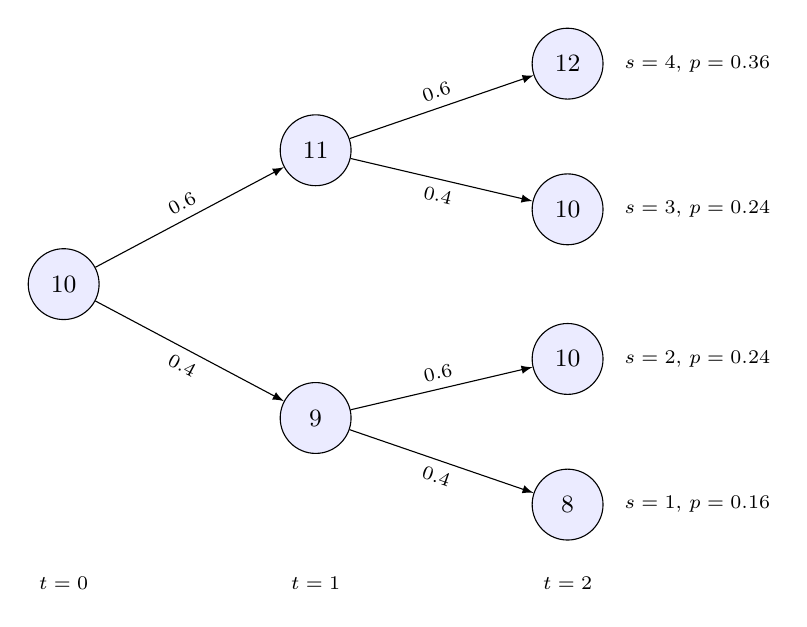
\begin{tikzpicture}[x=1cm,y=1cm,>=latex,font=\small,
  nd/.style={draw,circle,inner sep=1.4pt,minimum size=9mm,fill=blue!8},
  lb/.style={font=\scriptsize,midway,sloped,above}]
  \node[nd] (r)  at (0,0)      {$10$};
  \node[nd] (u)  at (3.2,1.7)  {$11$};
  \node[nd] (d)  at (3.2,-1.7) {$9$};
  \node[nd] (uu) at (6.4,2.8)  {$12$};
  \node[nd] (ud) at (6.4,0.95) {$10$};
  \node[nd] (du) at (6.4,-0.95){$10$};
  \node[nd] (dd) at (6.4,-2.8) {$8$};
  \draw[->] (r)  -- node[lb]{$0.6$} (u);
  \draw[->] (r)  -- node[lb,below]{$0.4$} (d);
  \draw[->] (u)  -- node[lb]{$0.6$} (uu);
  \draw[->] (u)  -- node[lb,below]{$0.4$} (ud);
  \draw[->] (d)  -- node[lb]{$0.6$} (du);
  \draw[->] (d)  -- node[lb,below]{$0.4$} (dd);
  \node[right,font=\scriptsize] at (7.0,2.8)  {$s = 4$, $p = 0.36$};
  \node[right,font=\scriptsize] at (7.0,0.95) {$s = 3$, $p = 0.24$};
  \node[right,font=\scriptsize] at (7.0,-0.95){$s = 2$, $p = 0.24$};
  \node[right,font=\scriptsize] at (7.0,-2.8) {$s = 1$, $p = 0.16$};
  \node[font=\scriptsize,below] at (0,-3.6)   {$t = 0$};
  \node[font=\scriptsize,below] at (3.2,-3.6) {$t = 1$};
  \node[font=\scriptsize,below] at (6.4,-3.6) {$t = 2$};
\end{tikzpicture}
\end{center}

\textbf{(b)(i) Extensive form.} Attach one decision to each \emph{node} of the
tree: $x_0$ at the root, $x_{1,1}$, $x_{1,2}$ at stage 1, and
$x_{2,1}, \ldots, x_{2,4}$ at stage 2, with the states $s$ indexed likewise.
Writing the cost of a node times the probability of reaching it,
\begin{align*}
\min\ & 10x_0
 + 0.4\left(9x_{1,1} + 0.4 \cdot 8 x_{2,1} + 0.6 \cdot 10 x_{2,2}\right)
 + 0.6\left(11x_{1,2} + 0.4 \cdot 10 x_{2,3} + 0.6 \cdot 12 x_{2,4}\right) \\
\text{s.t. } & s_0 = x_0, \\
& s_{1,1} = s_0 + x_{1,1}, \qquad s_{1,2} = s_0 + x_{1,2}, \\
& s_{2,1} = s_{1,1} + x_{2,1}, \quad s_{2,2} = s_{1,1} + x_{2,2}, \quad
  s_{2,3} = s_{1,2} + x_{2,3}, \quad s_{2,4} = s_{1,2} + x_{2,4}, \\
& s_{2,j} = a, \quad j = 1,\ldots,4, \\
& x \geq 0, \quad s \geq 0,
\end{align*}
where node $(1,1)$ carries $\xi_1 = 9$ and node $(1,2)$ carries $\xi_1 = 11$.

\textbf{(b)(ii) Scenario decomposition.} Attach instead one full decision path to
each \emph{scenario}: $x_t^{(s)}$ and $s_t^{(s)}$, $t = 0,1,2$, $s = 1,\ldots,4$.
With $p = (0.16, 0.24, 0.24, 0.36)$ and the cost paths $(10,9,8)$, $(10,9,10)$,
$(10,11,10)$, $(10,11,12)$,
\begin{align*}
\min\ & 0.16\left(10x_0^{(1)} + 9x_1^{(1)} + 8x_2^{(1)}\right)
      + 0.24\left(10x_0^{(2)} + 9x_1^{(2)} + 10x_2^{(2)}\right) \\
& + 0.24\left(10x_0^{(3)} + 11x_1^{(3)} + 10x_2^{(3)}\right)
  + 0.36\left(10x_0^{(4)} + 11x_1^{(4)} + 12x_2^{(4)}\right) \\
\text{s.t. } & s_0^{(s)} = x_0^{(s)}, \quad
 s_t^{(s)} = s_{t-1}^{(s)} + x_t^{(s)}, \quad t = 1,2, \quad s = 1,\ldots,4, \\
& s_2^{(s)} = a, \quad x_t^{(s)} \geq 0, \quad s_t^{(s)} \geq 0, \\
& x_0^{(1)} = x_0^{(2)} = x_0^{(3)} = x_0^{(4)}, & \text{(non-anticipativity, $t=0$)} \\
& x_1^{(1)} = x_1^{(2)}, \qquad x_1^{(3)} = x_1^{(4)}. & \text{(non-anticipativity, $t=1$)}
\end{align*}

\textbf{(c)} Only in the scenario decomposition. The extensive form attaches one
variable per \emph{node}, so two scenarios that are indistinguishable at time $t$
automatically share the same decision: non-anticipativity is built into the
indexing. The scenario decomposition duplicates the decisions along each path,
which is what makes the problem separable by scenario, and the coupling must
then be restored explicitly. Those are precisely the constraints that deck~08
dualizes, with multipliers $\pi$, and that progressive hedging enforces
iteratively.

Note the pattern: at $t = 2$ the four scenarios are all distinguishable, so no
constraint is needed; at $t = 1$ they form two groups; at $t = 0$ a single one.
\end{solution}

%%%%%%%%%%%%%%%%%%%%%%%%%%%%%%%%%%%%%%%%%%%%%%%%%%%%%%%%%%%%%%%%%%%%%%%%%%%%%%
\section{Monte Carlo approximation}
%%%%%%%%%%%%%%%%%%%%%%%%%%%%%%%%%%%%%%%%%%%%%%%%%%%%%%%%%%%%%%%%%%%%%%%%%%%%%%

\begin{exercise}
(Decks~03 and~09.) Show that
\[
\EE_{\bsxi}\left[ \min_{x \in \calX} z(x,\bsxi) \right] \leq \min_{x \in \calX} \EE_{\bsxi}\left[ z(x,\bsxi) \right]
\]
for a deterministic feasible set $\calX$. How is this result to be interpreted
for stochastic programming? Extend it to a Monte Carlo sample average.
\end{exercise}

\begin{solution}
Assume the expectations are well defined and the minima attained, as the
statement implicitly does. There exists $x^* \in \calX$ with
$\min_{x \in \calX} \EE_{\bsxi}[z(x,\bsxi)] = \EE_{\bsxi}[z(x^*,\bsxi)]$. Since
$x^* \in \calX$,
\[
\min_{x \in \calX} z(x,\xi) \leq z(x^*,\xi) \quad \text{for every } \xi,
\]
and taking expectations gives the result.

Without attainment the statement still holds with infima: for every
$y \in \calX$, $\inf_{x \in \calX} z(x,\bsxi) \leq z(y,\bsxi)$, hence
$\EE_{\bsxi}[\inf_{x \in \calX} z(x,\bsxi)] \leq \EE_{\bsxi}[z(y,\bsxi)]$, and
taking the infimum over $y$ closes the argument.

\textbf{Interpretation.} This is $\WSv \leq \RPv$ of deck~03: minimizing under
perfect information is optimistic. A decision tailored to each realization can
only beat a single decision that must serve them all.

\textbf{Extension to sampling.} Let
$z_N(x) = \frac{1}{N}\sum_{n=1}^N z(x,\bsxi_n)$ be the sample average over an
i.i.d.\ sample. The result just proved applies verbatim with the random element
taken to be the whole sample $(\bsxi_1,\ldots,\bsxi_N)$ and the function
$z_N$ in place of $z$:
\[
\EE\left[ \min_{x \in \calX} z_N(x) \right]
\ \leq\ \min_{x \in \calX} \EE\left[ z_N(x) \right]
\ =\ \min_{x \in \calX} \EE_{\bsxi}\left[ z(x,\bsxi) \right],
\]
the last equality because $z_N(x)$ is an unbiased estimator of
$\EE_{\bsxi}[z(x,\bsxi)]$ for each fixed $x$.

\medskip
\emph{Caution.} One cannot argue by exchanging the minimum and the sum, writing
$\min_x \frac{1}{N}\sum_n z(x,\bsxi_n) = \frac{1}{N}\sum_n \min_x z(x,\bsxi_n)$:
the minimum of a sum is not the sum of the minima, and the inequality in fact
runs the other way,
\[
\min_{x \in \calX} \frac{1}{N}\sum_{n=1}^N z(x,\bsxi_n)
\ \geq\ \frac{1}{N}\sum_{n=1}^N \min_{x \in \calX} z(x,\bsxi_n),
\]
since a single $x$ must serve all $N$ draws. That route does not close the chain;
the one above does.

\medskip
The conclusion is that the sample-average optimal value is a
\emph{downward-biased} estimator of the true optimal value: the optimizer
exploits the particular sample it was given. This is the bias that deck~09
analyses, and why an out-of-sample evaluation is needed to obtain an honest upper
bound.
\end{solution}

\end{document}
"
% The Makefile target `exercises` builds both. Nothing has to be kept in sync.
\newif\ifsolutions
\solutionstrue
\ifdefined\nosolutions\solutionsfalse\fi

\newcounter{exercisecount}[section]
\renewcommand{\theexercisecount}{\thesection.\arabic{exercisecount}}
\newenvironment{exercise}
  {\par\medskip\refstepcounter{exercisecount}%
   \noindent\textbf{Exercise \theexercisecount.}\begin{itshape}}
  {\end{itshape}\par\medskip}

\ifsolutions
  \newenvironment{solution}
    {\par\nobreak\smallskip\noindent\textbf{Solution.}\par\nobreak\smallskip}
    {\par\medskip\hrule height 0pt\medskip}
\else
  \excludecomment{solution}
\fi

\newcommand{\WSv}{\mathrm{WS}}
\newcommand{\RPv}{\mathrm{RP}}
\newcommand{\EVv}{\mathrm{EV}}
\newcommand{\EEVv}{\mathrm{EEV}}
\newcommand{\EVPIv}{\mathrm{EVPI}}
\newcommand{\VSSv}{\mathrm{VSS}}

\title{Stochastic optimization\\[2mm] \Large Exercise collection%
\ifsolutions\\[2mm]\normalsize with solutions\fi}
\author{Fabian Bastin\\ \small Université de Montréal -- CIRRELT -- IVADO}
\date{}

\begin{document}

\maketitle

\noindent
This collection accompanies the lecture slides. Each exercise names the deck it
depends on.
\ifsolutions
This is the version \emph{with solutions}; the statements alone are in
\texttt{exercises.pdf}.
\else
This version holds the \emph{statements only}; the solutions are in
\texttt{exercises\_solutions.pdf}.
\fi

\medskip
\noindent
Sources are indicated exercise by exercise; several are adapted from Birge and
Louveaux, \emph{Introduction to Stochastic Programming}, 2nd edition, Springer,
2011.

\tableofcontents

%%%%%%%%%%%%%%%%%%%%%%%%%%%%%%%%%%%%%%%%%%%%%%%%%%%%%%%%%%%%%%%%%%%%%%%%%%%%%%
\section{Generalities}
%%%%%%%%%%%%%%%%%%%%%%%%%%%%%%%%%%%%%%%%%%%%%%%%%%%%%%%%%%%%%%%%%%%%%%%%%%%%%%

\begin{exercise}
(Deck~03.) Show that the value of the stochastic solution and the expected value
of perfect information are always non-negative.
\end{exercise}

\begin{solution}
Consider the general problem $\min_{x \in X} \EE[z(x,\bsxi)]$, and recall the
four quantities
\[
\RPv = \min_{x \in X} \EE[z(x,\bsxi)], \qquad
\WSv = \EE\left[ \min_{x \in X} z(x,\bsxi) \right], \qquad
\EVv = \min_{x \in X} z(x, \overline{\xi}), \quad \overline{\xi} = \EE[\bsxi],
\]
and
\[
\EEVv = \EE\left[ z\!\left(\overline{x}(\overline{\xi}), \bsxi\right) \right],
\qquad \overline{x}(\overline{\xi}) \in \arg\min_{x \in X} z(x,\overline{\xi}).
\]

\emph{A warning on $\EEVv$.} It is \textbf{not} $\EE[\EVv]$: $\EVv$ is a
deterministic number, so $\EE[\EVv] = \EVv$. $\EEVv$ is the expected cost of
\emph{using} the expected-value decision, the uncertainty being restored
afterwards. This is exactly what makes $\VSSv$ measure something.

\medskip
$\VSSv = \EEVv - \RPv \geq 0$. Since $\overline{x}(\overline{\xi}) \in X$, it is
one particular feasible point of the recourse problem, so
\[
\RPv = \min_{x \in X} \EE[z(x,\bsxi)] \leq \EE\left[z\!\left(\overline{x}(\overline{\xi}),\bsxi\right)\right] = \EEVv .
\]

\medskip
$\EVPIv = \RPv - \WSv \geq 0$. Let $x^*_{\RPv} \in \arg\min_{x \in X} \EE[z(x,\bsxi)]$.
For every realization $\xi$,
\[
z(x^*_{\RPv}, \xi) \geq \min_{x \in X} z(x,\xi),
\]
and taking expectations, which preserves inequalities,
\[
\RPv = \EE\left[z(x^*_{\RPv},\bsxi)\right] \geq \EE\left[\min_{x \in X} z(x,\bsxi)\right] = \WSv .
\]

\medskip
Both arguments have the same shape: a single decision that must serve every
realization can only be worse than a decision tailored to each one.
\end{solution}

%%%%%%%%%%%%%%%%%%%%%%%%%%%%%%%%%%%%%%%%%%%%%%%%%%%%%%%%%%%%%%%%%%%%%%%%%%%%%%
\section{Two-stage problems with recourse}
%%%%%%%%%%%%%%%%%%%%%%%%%%%%%%%%%%%%%%%%%%%%%%%%%%%%%%%%%%%%%%%%%%%%%%%%%%%%%%

\begin{exercise}
(Deck~01 and~03.) Consider the farmer problem of deck~01. Is its recourse
\emph{complete}? \emph{Relatively complete}? \emph{Simple}?
\end{exercise}

\begin{solution}
Write $t_1$, $t_2$, $t_3$ for the yields (tons per acre) of one scenario, $y_1$,
$y_2$ for the tons of wheat and corn bought, $w_1$, $w_2$ for the tons sold, and
$w_3$, $w_4$ for the tons of sugar beets sold at the high and at the low price.
Given the acreages $x$, the second stage is
\begin{align*}
\min_{y,w}\ & 238y_1 - 170w_1 + 210y_2 - 150w_2 - 36w_3 - 10w_4 \\
\text{s.t. } & t_1x_1 + y_1 - w_1 \geq 200, \qquad t_2x_2 + y_2 - w_2 \geq 240, \\
& w_3 + w_4 \leq t_3x_3, \qquad w_3 \leq 6000, \qquad y, w \geq 0.
\end{align*}
Adding slacks $s \geq 0$ and moving $x$ to the right-hand side,
\[
y_1 - w_1 - s_1 = 200 - t_1x_1, \quad
y_2 - w_2 - s_2 = 240 - t_2x_2, \quad
w_3 + w_4 + s_3 = t_3x_3, \quad
w_3 + s_4 = 6000,
\]
so that, with the columns ordered as $(y_1, y_2, w_1, w_2, w_3, w_4, s_1, s_2, s_3, s_4)$,
\[
W = \begin{pmatrix}
1 & 0 & -1 & 0 & 0 & 0 & -1 & 0 & 0 & 0 \\
0 & 1 & 0 & -1 & 0 & 0 & 0 & -1 & 0 & 0 \\
0 & 0 & 0 & 0 & 1 & 1 & 0 & 0 & 1 & 0 \\
0 & 0 & 0 & 0 & 1 & 0 & 0 & 0 & 0 & 1
\end{pmatrix}.
\]

\textbf{Not complete.} Rows 3 and 4 meet only columns with non-negative entries,
so every $z \in \operatorname{pos} W$ has $z_3 \geq 0$ and $z_4 \geq 0$.
Conversely any such $z$ is attained (take $w_3 = 0$, $s_4 = z_4$, $w_4 = z_3$,
$s_3 = 0$, and use $(y_1,w_1)$, $(y_2,w_2)$ for the first two rows, which are
unrestricted). Hence
$\operatorname{pos} W = \RR \times \RR \times \RR_+ \times \RR_+ \neq \RR^4$.

\textbf{Relatively complete.} We need $h(\xi) - T(\xi)x \in \operatorname{pos} W$
for every $x \in K_1 = \lbrace x \in \RR^3_+ \mid x_1+x_2+x_3 \leq 500 \rbrace$
and every scenario. Its third and fourth components are $t_3x_3$ and $6000$,
both non-negative since $x_3 \geq 0$ and the yields are positive. So
$K_1 \subseteq K_2$. Concretely, buying all the wheat and corn needed and selling
no sugar beets is feasible whatever the seeding decision and the yields ---
expensive, but feasible.

\textbf{Not simple.} Simple recourse requires $W = \begin{pmatrix} I & -I \end{pmatrix}$.
Here $W$ is $4 \times 10$ and $w_3$ appears in two rows, the quota coupling the
beet sales to the harvest.

\medskip
Completeness is read off $W$ alone and fails here on a technicality; relative
completeness --- the property that matters --- holds because every right-hand
side the model can produce lands in $\operatorname{pos} W$.
\end{solution}

\begin{exercise}
(Deck~03; Birge and Louveaux, p.~87.) Consider the second-stage program
\[
Q(x,\xi) = \min_y \lbrace y \mid \xi y = 1-x,\ y \geq 0 \rbrace,
\]
where $\bsxi$ follows a triangular distribution on $[0,1]$, i.e.\ $P[\bsxi \leq u] = u^2$.
\begin{enumerate}[(a)]
\item Is the recourse fixed? Why?
\item Express $K_2(\xi)$ for every $\xi \in [0,1]$.
\item Express $K_2$, $K_2^P$ and $\calQ$.
\end{enumerate}
\end{exercise}

\begin{solution}
\textbf{(a)} The recourse is \emph{not} fixed: here $W \equiv \bsxi$, which is
random. Moreover $\xi$ can take the value $0$, so the transformation
$y = (1-x)/\xi$ is not defined on all of $\Xi = [0,1]$. In terms of the cone,
\[
\operatorname{pos} W =
\begin{cases}
\lbrace 0 \rbrace & \text{if } \xi = 0, \\
\RR_+ & \text{if } \xi \neq 0.
\end{cases}
\]

\textbf{(b)} Two cases.
\emph{$\xi \in (0,1]$:} since $y \geq 0$ and $\xi > 0$, feasibility requires
$1-x \geq 0$, so $K_2(\xi) = \lbrace x \mid x \leq 1 \rbrace$, with
$Q(x,\xi) = (1-x)/\xi$ attained at $y^* = (1-x)/\xi$.
\emph{$\xi = 0$:} no $y$ satisfies $0 \cdot y = 1-x$ unless $x = 1$, so
$K_2(0) = \lbrace 1 \rbrace$.

\textbf{(c)} Therefore
\[
K_2^P = \lbrace x \mid x \leq 1 \rbrace \cap \lbrace 1 \rbrace = \lbrace 1 \rbrace,
\]
while, since $P[\bsxi = 0] = 0$ and the density is $f(\xi) = 2\xi$,
\[
\calQ(x) = \int_0^1 \frac{1-x}{\xi}\, 2\xi \, d\xi = 2(1-x), \qquad \forall x \leq 1,
\]
so $K_2 = \lbrace x \mid x \leq 1 \rbrace$ and $K_2^P \subsetneq K_2$.

\medskip
The difference is that a point leaves $K_2^P$ as soon as it is infeasible for
\emph{one} value of $\xi$, whatever its probability, whereas $K_2$ ignores
infeasibilities occurring with probability zero. Recall that for a program with
a \emph{fixed} recourse --- not the case here --- and $\bsxi$ with finite
second-order moments, we would have had $K_2 = K_2^P$.
\end{solution}

\begin{exercise}
(Deck~03.) Consider the second-stage program
\begin{align*}
\min_y\ & 2y_1+y_2\\
\text{s.t. } & y_1 - y_2 \leq 2-\bsxi x_1,\\
& y_2 \leq x_2,\\
& y_1, y_2 \geq 0.
\end{align*}
Find $K_2(\xi)$ and $K_2$ when (a) $\bsxi \sim U[0,1]$; (b) $\bsxi \sim \text{Poisson}(\lambda)$, $\lambda > 0$.
Which properties do you expect of $K_2$? Is the recourse simple or complete? If
not, under which conditions would it be relatively complete?
\end{exercise}

\begin{solution}
\textbf{The elementary set.} $y_2 \geq 0$ and $y_2 \leq x_2$ force $x_2 \geq 0$.
The first constraint then reads $y_1 \leq 2 - \xi x_1 + y_2$, and the largest
admissible right-hand side is obtained at $y_2 = x_2$; a feasible $y_1 \geq 0$
exists if and only if $2 - \xi x_1 + x_2 \geq 0$. Hence
\[
K_2(\xi) = \lbrace x \mid x_2 \geq 0,\ \xi x_1 \leq 2+x_2 \rbrace
= \lbrace x \mid x_2 \geq \max(0, \xi x_1 - 2) \rbrace .
\]

\textbf{(a) $\bsxi \sim U[0,1]$}, $\Xi = [0,1]$. The recourse is fixed ($\bsxi$
enters only through $T(\bsxi)$) and the distribution has finite second-order
moments, so $K_2 = K_2^s = K_2^P = \bigcap_{\xi \in \Xi} K_2(\xi)$.
For $x_1 \geq 0$ and $\xi \leq 1$, $\xi x_1 \leq x_1$, so
$x \in K_2(1) \Rightarrow x \in K_2(\xi)$; for $x_1 < 0$, $\xi x_1 \leq 0 \leq 2+x_2$
always. In both cases $K_2(1) \subseteq K_2(\xi)$ for every $\xi \in \Xi$: the
intersection is reached at $\xi = 1$ and
\[
K_2 = \lbrace x \mid x_2 \geq 0,\ x_1 \leq 2+x_2 \rbrace .
\]

\textbf{(b) $\bsxi \sim \text{Poisson}(\lambda)$}, $\Xi = \lbrace 0,1,2,\ldots\rbrace$
unbounded. If $x_1 > 0$ then $\xi x_1$ is unbounded above and no $x_2$ absorbs
it; if $x_1 \leq 0$ then $\xi x_1 \leq 0 \leq 2+x_2$. Hence
$K_2 = \lbrace x \mid x_1 \leq 0,\ x_2 \geq 0 \rbrace$.

\textbf{Expected properties.} Each $K_2(\xi)$ is an intersection of two
half-spaces, hence closed and convex, and so is $K_2$. This is no accident: with
a fixed recourse $x \in K_2(\xi) \iff h(\xi)-T(\xi)x \in \operatorname{pos} W$,
and $\operatorname{pos} W$ is a closed convex cone. With a finite support $K_2$
would moreover be polyhedral; here $\Xi$ is infinite, yet both answers happen to
be polyhedral.

\textbf{Type of recourse.} Putting the program in standard form with surplus
variables $s_1, s_2 \geq 0$,
\[
y_1 - y_2 + s_1 = 2 - \xi x_1, \qquad y_2 + s_2 = x_2,
\qquad
W = \begin{pmatrix} 1 & -1 & 1 & 0 \\ 0 & 1 & 0 & 1 \end{pmatrix}.
\]
The recourse is \emph{not simple} ($W$ is not $\begin{pmatrix} I & -I\end{pmatrix}$),
and \emph{not complete}: the second row involves only non-negative coefficients,
so $z_2 < 0$ is unreachable and $\operatorname{pos} W = \RR \times \RR_+ \neq \RR^2$.
It is \emph{relatively complete} exactly when $K_1 \subseteq K_2$, i.e.\ when the
first stage already enforces $x_2 \geq 0$ together with $x_1 \leq 2+x_2$ in
case~(a), or $x_1 \leq 0$ in case~(b). If the first stage merely requires
$x \geq 0$, then
\[
\text{(a)}\quad K_1 \cap K_2 \subseteq \lbrace x \geq 0 \mid x_1 \leq 2+x_2 \rbrace,
\qquad
\text{(b)}\quad K_1 \cap K_2 \subseteq \lbrace x \mid x_1 = 0,\ x_2 \geq 0 \rbrace .
\]
Relative completeness is plausible in the first case and very restrictive in the
second: an unbounded support is far less forgiving, since \emph{every}
realization has to be survived.
\end{solution}

\begin{exercise}
(Deck~03; Birge and Louveaux, p.~102.) Consider the second-stage program
\begin{align*}
\min_y\ & 2y_1+y_2\\
\text{s.t. } & y_1 + y_2 \geq 1-x_1,\\
& y_1 \geq \bsxi - x_1-x_2,\\
& y_1, y_2 \geq 0.
\end{align*}
Show that this program has a complete recourse when $\bsxi$ has a finite expectation.
\end{exercise}

\begin{solution}
\textbf{A direct argument.} Completeness asks that for every right-hand side
$(z_1, z_2)$ there exist $y_1, y_2 \geq 0$ with $y_1 + y_2 \geq z_1$ and
$y_1 \geq z_2$. Taking $y_1 = \max\lbrace 0, z_2 \rbrace$ satisfies the second,
and $y_2 = \max\lbrace 0, z_1 - y_1 \rbrace$ the first; both are non-negative.

\textbf{Through $\operatorname{pos} W$.} The standard characterisation requires
$Wy = z$ with $y \geq 0$, and is stated for equalities: showing that $Wy \geq z$
is solvable is \emph{not} the same statement. So bring the program to the
standard form first, with surplus variables $s \geq 0$:
\[
y_1 + y_2 - s_1 = 1-x_1, \qquad y_1 - s_2 = \xi - x_1 - x_2,
\qquad
W = \begin{pmatrix} 1 & 1 & -1 & 0 \\ 1 & 0 & 0 & -1 \end{pmatrix}.
\]
The second row leaves $y_1$ free to absorb the sign of $z_2$:
\[
\begin{cases}
y_1 = z_2,\ s_2 = 0 & \text{if } z_2 \geq 0,\\
y_1 = 0,\ s_2 = -z_2 & \text{otherwise.}
\end{cases}
\]
The first row then reads $y_2 - s_1 = z_1 - y_1$. If $z_2 \geq 0$, then
$y_2 - s_1 = z_1 - z_2$ and we take
\[
\begin{cases}
y_2 = z_1-z_2,\ s_1 = 0 & \text{if } z_1-z_2 \geq 0,\\
y_2 = 0,\ s_1 = z_2-z_1 & \text{otherwise;}
\end{cases}
\]
if $z_2 < 0$, then $y_1 = 0$, $y_2 - s_1 = z_1$, and it suffices to choose
\[
\begin{cases}
y_2 = z_1,\ s_1 = 0 & \text{if } z_1 \geq 0,\\
y_2 = 0,\ s_1 = -z_1 & \text{otherwise.}
\end{cases}
\]
Every $z \in \RR^2$ is reached, so $\operatorname{pos} W = \RR^2$ and the
recourse is complete.

\textbf{The hypothesis on $\EE[\bsxi]$ played no role}, and could not have:
completeness involves only $W$, which is fixed. The statement is copied from
Birge and Louveaux, where the hypothesis is superfluous at this point. In
particular it is \emph{not} what gives $K_2 = \RR^2$ --- completeness alone does.

What a finite expectation buys is the \emph{finiteness} of the recourse. Deck~03
uses exactly this $W$ with $P[\bsxi = 2^n] = 2^{-(n+1)}$, $n = 0,1,2,\ldots$, for
which $\EE[\bsxi] = +\infty$, to exhibit a problem where the recourse is complete
--- hence $K_2 = \RR^2$ --- while $\calQ(x) = +\infty$ everywhere, so
$K_2^s = \emptyset$. Complete recourse and finite recourse are two different
things.
\end{solution}

\begin{exercise}
(Deck~03.) A company must order a quantity $x$ of a product to meet a demand $d$
that is unknown at the time of ordering. The unit ordering cost is $c > 0$. If
$d > x$, a penalty $b \geq 0$ is incurred per unit of unmet demand; if $d < x$,
a holding cost $h$ is incurred per surplus unit.
\begin{enumerate}[(a)]
\item Formulate the problem as a two-stage stochastic program.
\item Is the recourse simple, complete, relatively complete?
\item What can be expected of the first-stage solution when $b < c$?
\end{enumerate}
\end{exercise}

\begin{solution}
\textbf{(a)} The first stage is the order; the second stage settles the
discrepancy between $x$ and the realized demand:
\[
\min_{x \geq 0}\ cx + \EE_{\bsd}[Q(x,\bsd)],
\qquad
Q(x,d) = \min_{y^+,y^- \geq 0} \lbrace by^+ + hy^- \mid y^+ - y^- = d-x \rbrace .
\]

\textbf{(b)} Here $W = \begin{pmatrix} 1 & -1 \end{pmatrix}$, so the recourse is
\emph{simple}, hence also complete and relatively complete. The finiteness
condition of the simple-recourse theorem reads $b + h \geq 0$, satisfied as soon
as both costs are non-negative.

\textbf{(c)} With $b < c$, an extra ordered unit costs more than the penalty it
avoids. Formally, the objective $cx + \EE[b(\bsd-x)^+ + h(x-\bsd)^+]$ has
right derivative at $x$ equal to $c - b\,P[\bsd > x] + h\,P[\bsd < x] \geq c - b > 0$,
so the objective is strictly increasing and $x^* = 0$: the company orders
nothing and pays the penalty.
\end{solution}

\begin{exercise}
(Deck~03.) A good $X$ must be produced before its demand is known. Each unit
produced costs \$2. Demand is discrete, taking the values $D_s$ with
probabilities $p_s$, $s = 1,\ldots,S$. Demand can also be met by buying from an
external supplier at \$3 per unit, once it has been observed. How much should be
produced now? Formulate the problem as a two-stage stochastic program minimizing
the expected production cost.
\end{exercise}

\begin{solution}
Let $x \geq 0$ be the number of units produced at the first stage, and
$y_s \geq 0$ the number bought from the external supplier in scenario $s$. Demand
is met when $x + y_s \geq D_s$, so
\begin{align*}
\min\ & 2x + \sum_{s=1}^S p_s\, 3 y_s \\
\text{s.t. } & x + y_s \geq D_s, \quad s = 1,\ldots,S, \\
& x \geq 0, \quad y_s \geq 0, \quad s = 1,\ldots,S.
\end{align*}
The second stage decomposes scenario by scenario, with $y_s = (D_s - x)^+$, so
the model is a simple-recourse one: producing is cheaper than outsourcing, but
must be committed to before the demand is known.
\end{solution}

\begin{exercise}
(Deck~03; Higle, \emph{Tutorials in Operations Research}, INFORMS, 2005.)
The Dakota Furniture Company makes desks, tables and chairs. Each item consumes
lumber and two kinds of skilled labour, finishing and carpentry:

\begin{center}
\begin{tabular}{|l|c|c|c|c|}
\hline
Resource & Cost & Desk & Table & Chair \\
\hline
Lumber (board ft.) & \$2 & 8 & 6 & 1 \\
Finishing (hours)  & \$4 & 4 & 2 & 1.5 \\
Carpentry (hours)  & \$5.2 & 2 & 1.5 & 0.5 \\
\hline
Selling price & & \$60 & \$40 & \$10 \\
\hline
\end{tabular}
\end{center}

Resources must be acquired before the demand is known. Three equally structured
demand scenarios are considered, with probabilities $0.3$, $0.4$ and $0.3$:

\begin{center}
\begin{tabular}{|l|c|c|c|}
\hline
Scenario & Desks & Tables & Chairs \\
\hline
Low ($p = 0.3$)         & 50  & 20  & 200 \\
Most likely ($p = 0.4$) & 150 & 110 & 225 \\
High ($p = 0.3$)        & 250 & 250 & 500 \\
\hline
\end{tabular}
\end{center}

Formulate the problem as a two-stage stochastic program maximizing the expected
profit. Only the formulation is asked.
\end{exercise}

\begin{solution}
Treat it as a resource-allocation problem. First stage: $x_1$ board feet of
lumber, $x_2$ finishing hours, $x_3$ carpentry hours. Second stage: $y_1$ desks,
$y_2$ tables, $y_3$ chairs produced once the demand is known.
\[
\min_{x \geq 0}\ 2x_1 + 4x_2 + 5.2x_3 + \EE_{\bsxi}[Q(x,\bsxi)],
\]
with
\begin{align*}
Q(x,\xi) = \min_y\ & -60y_1 - 40y_2 - 10y_3 \\
\text{s.t. } & 8y_1 + 6y_2 + y_3 \leq x_1, \\
& 4y_1 + 2y_2 + 1.5y_3 \leq x_2, \\
& 2y_1 + 1.5y_2 + 0.5y_3 \leq x_3, \\
& y_i \leq d_i(\xi),\ i = 1,2,3, \qquad y \geq 0 .
\end{align*}
Maximizing profit is minimizing its negative, hence the signs in $Q$. With the
three scenarios,
\[
\EE_{\bsxi}[Q(x,\bsxi)] = 0.3\,Q(x,\xi_1) + 0.4\,Q(x,\xi_2) + 0.3\,Q(x,\xi_3),
\]
where $d(\xi_1) = (50,20,200)$, $d(\xi_2) = (150,110,225)$ and
$d(\xi_3) = (250,250,500)$.
\end{solution}

\begin{exercise}
(Deck~03; Birge and Louveaux, p.~142.) Consider
\begin{align*}
\min_x\ & x_1 + 4x_2 + \EE_{\bsxi}[Q(x,\bsxi)] \\
\text{s.t. } & x_1 + x_2 = 1, \quad x \geq 0,
\end{align*}
with
\begin{align*}
Q(x,\xi) = \min_y\ & y_1 + 10y_2 + 10y_3 \\
\text{s.t. } & y_1 + y_2 - y_3 = \xi + x_1 - 2x_2, \\
& y_1 \leq 2, \qquad y \geq 0,
\end{align*}
and $\bsxi \sim U[1,3]$.
\begin{enumerate}[(a)]
\item Is the recourse fixed, simple, complete, relatively complete? Answer true
or false for each, with a brief justification.
\item For given $x$ and $\xi$, show, by discussing the value of $\xi + x_1 - 2x_2$, that
\[
y^*(x,\xi) =
\begin{cases}
y_1 = \xi + x_1 - 2x_2,\ y_2 = y_3 = 0 & \text{if } 0 \leq \xi + x_1 - 2x_2 \leq 2,\\
y_1 = 2,\ y_2 = \xi + x_1 - 2x_2 - 2,\ y_3 = 0 & \text{if } \xi + x_1 - 2x_2 > 2,\\
y_3 = 2x_2 - \xi - x_1,\ y_1 = y_2 = 0 & \text{if } \xi + x_1 - 2x_2 < 0.
\end{cases}
\]
\item Which expected property of $Q(x,\xi)$ does $y^*(x,\xi)$ confirm?
\item Is $\calQ(x) = \EE_{\bsxi}[Q(x,\bsxi)]$ differentiable? Why?
\item Express $K_1$, $K_2(\xi)$, $K_2^P$ and $K_2$.
\item Give the deterministic equivalent (extensive form) of the discretized
problem where $\bsxi$ takes the values $1$, $2$, $3$.
\end{enumerate}
\end{exercise}

\begin{solution}
\textbf{(a)} Adding a slack $y_4$ to the second constraint puts the second stage
in standard form,
\[
y_1 + y_2 - y_3 = \xi + x_1 - 2x_2, \qquad y_1 + y_4 = 2,
\qquad
W = \begin{pmatrix} 1 & 1 & -1 & 0 \\ 1 & 0 & 0 & 1 \end{pmatrix}.
\]
\emph{Fixed}: true, $W$ does not depend on $\xi$.
\emph{Simple}: false, $W$ is not of the form $\begin{pmatrix} I & -I\end{pmatrix}$.
\emph{Complete}: false --- the second row reads $y_1 + y_4 = z_2$ with
$y_1, y_4 \geq 0$, so no $z_2 < 0$ is reachable.
\emph{Relatively complete}: true. For any $x \in K_1$ and any $\xi$, the point
\[
y_1 = 0, \quad y_2 = (\xi + x_1 - 2x_2)^+, \quad y_3 = (-\xi - x_1 + 2x_2)^+, \quad y_4 = 2
\]
is feasible, the second component of the right-hand side being the constant $2 \geq 0$.

\textbf{(b)} Write $d = \xi + x_1 - 2x_2$. If $d < 0$, the only feasible extreme
point is $y_1 = y_2 = 0$, $y_3 = -d$, $y_4 = 2$, hence optimal. If $d \geq 0$,
an extreme point has $y_3 = 0$ and $y_1 + y_2 = d$ with $y_1 \leq 2$. Since the
cost of $y_1$ is $1$ and that of $y_2$ is $10$, $y_1$ is pushed as far as
possible: $y_1 = \min\lbrace d, 2 \rbrace$. This splits into $d \leq 2$, giving
$y_1 = d$, $y_2 = 0$, and $d \geq 2$, giving $y_1 = 2$, $y_2 = d-2$, as announced.

\textbf{(c)} $Q(\cdot,\xi)$ is convex and piecewise linear in the first-stage
decision $x$: the three regimes above are the three linear pieces, with
breakpoints where $d = 0$ and $d = 2$.

\textbf{(d)} Yes. $\bsxi$ is continuous with an absolutely continuous
distribution and finite second-order moments, so $\calQ$ is differentiable on the
interior of $K_2$: integrating over $\xi$ smooths away the kinks of each
$Q(\cdot,\xi)$.

\textbf{(e)} Directly from the statement,
$K_1 = \lbrace x \mid x_1 + x_2 = 1,\ x \geq 0 \rbrace$.
From (b), the second stage is feasible whatever $d$, so
$K_2(\xi) = \RR^2$ for every $\xi$, and therefore
$K_2^P = \bigcap_{\xi \in \Xi} K_2(\xi) = \RR^2$ and $K_2 = \RR^2$ as well.
In particular $K_1 \subseteq K_2$, confirming (a).

\textbf{(f)} With $\xi_1 = 1$, $\xi_2 = 2$, $\xi_3 = 3$ and $p_i = 1/3$,
\begin{align*}
\min\ & x_1 + 4x_2 + \sum_{i=1}^3 p_i\left(y_{1i} + 10y_{2i} + 10y_{3i}\right) \\
\text{s.t. } & x_1 + x_2 = 1, \\
& y_{1i} + y_{2i} - y_{3i} = \xi_i + x_1 - 2x_2, \quad i = 1,2,3, \\
& y_{1i} \leq 2, \quad i = 1,2,3, \\
& x \geq 0, \quad y_{1i}, y_{2i}, y_{3i} \geq 0, \quad i = 1,2,3.
\end{align*}
\end{solution}

%%%%%%%%%%%%%%%%%%%%%%%%%%%%%%%%%%%%%%%%%%%%%%%%%%%%%%%%%%%%%%%%%%%%%%%%%%%%%%
\section{Decomposition methods}
%%%%%%%%%%%%%%%%%%%%%%%%%%%%%%%%%%%%%%%%%%%%%%%%%%%%%%%%%%%%%%%%%%%%%%%%%%%%%%

\begin{exercise}
(Deck~04.) Consider
\begin{align*}
\min\ & 100x_1 + 150x_2 + \EE_{\bsxi}[q_1y_1 + q_2y_2] \\
\text{s.t. } & x_1 + x_2 \leq 120, \\
& 6y_1 + 10y_2 \leq 60x_1, \qquad 8y_1 + 5y_2 \leq 80x_2, \\
& y_1 \leq d_1, \qquad y_2 \leq d_2, \\
& x_1 \geq 40,\ x_2 \geq 20, \qquad y_1, y_2 \geq 0,
\end{align*}
under two scenarios $\bsxi = (d_1, d_2, q_1, q_2)$: $\xi_1 = (500, 100, -24, -28)$
with probability $p_1 = 0.4$, and $\xi_2 = (300, 300, -28, -32)$ with
probability $p_2 = 0.6$.

Run the first iteration of the single-cut $L$-shaped method, showing that the
second-stage solutions are respectively $y^* = (137.5, 100)$ and
$y^* = (80, 192)$. To obtain the dual solutions, use complementary slackness: a
dual variable can be non-zero only if the associated primal constraint is active.
\end{exercise}

\begin{solution}
\textbf{Master problem.} With no cut yet,
$\min \lbrace 100x_1 + 150x_2 \mid x_1 + x_2 \leq 120,\ x_1 \geq 40,\ x_2 \geq 20 \rbrace$,
whose optimal solution is immediately $x^1 = (40, 20)$, so $60x_1 = 2400$ and
$80x_2 = 1600$.

Since $x_1, x_2 \geq 0$ makes the second stage always feasible, the recourse is
relatively complete and no feasibility cut is needed.

\textbf{First scenario.}
$\min -24y_1 - 28y_2$ s.t. $6y_1 + 10y_2 \leq 2400$, $8y_1 + 5y_2 \leq 1600$,
$y_1 \leq 500$, $y_2 \leq 100$, $y \geq 0$.
We cannot have $y_1 = 500$, as the second constraint would be violated.
Setting $y_2 = 100$,
\[
y_1 = \min\left\lbrace \frac{2400-1000}{6},\ \frac{1600-500}{8} \right\rbrace
= \min\left\lbrace \frac{1400}{6},\ \frac{1100}{8} \right\rbrace
= \min\left\lbrace 233.33,\ 137.5 \right\rbrace = 137.5 .
\]
The alternative, making the first two constraints active, solves
$3y_1 + 5y_2 = 1200$ and $8y_1 + 5y_2 = 1600$, giving $y_1 = 80$, $y_2 = 192$,
which violates $y_2 \leq 100$. Hence $y^* = (137.5, 100)$, with objective
$-6100$.

Active constraints: the second and $y_2 \leq 100$. Complementary slackness gives
$\pi_1^* = \pi_3^* = 0$, and both $y_1, y_2 > 0$ make the dual constraints tight:
\[
8\pi_2^* = -24 \ \Rightarrow\ \pi_2^* = -3,
\qquad
5\pi_2^* + \pi_4^* = -28 \ \Rightarrow\ \pi_4^* = -28 + 15 = -13 .
\]

\textbf{Second scenario.}
$\min -28y_1 - 32y_2$, same first two constraints, $y_1 \leq 300$, $y_2 \leq 300$.
Taking $y_1 = 300$ or $y_2 = 300$ violates one of the first two constraints, so
both are active:
\[
3y_1 + 5y_2 = 1200, \qquad 8y_1 + 5y_2 = 1600
\ \Longrightarrow\ y^* = (80, 192),
\]
with objective $-8384$. Then $\pi_3^* = \pi_4^* = 0$ and
\[
6\pi_1^* + 8\pi_2^* = -28, \qquad 10\pi_1^* + 5\pi_2^* = -32 .
\]
Multiplying the first by $5$ and the second by $8$ and subtracting,
$50\pi_1^* = -116$, so $\pi_1^* = -2.32$; then
$5\pi_2^* = -32 + 23.2 = -8.8$, so $\pi_2^* = -1.76$.

\textbf{Optimality cut.} Writing the second-stage constraints as
$Wy \leq h(\xi) - T(\xi)x$,
\[
h(\xi_1) = \begin{pmatrix} 0 \\ 0 \\ 500 \\ 100 \end{pmatrix}, \quad
h(\xi_2) = \begin{pmatrix} 0 \\ 0 \\ 300 \\ 300 \end{pmatrix}, \quad
T(\xi_1) = T(\xi_2) = T = \begin{pmatrix} -60 & 0 \\ 0 & -80 \\ 0 & 0 \\ 0 & 0 \end{pmatrix}.
\]
Hence
\[
e_1 = 0.4\,\pi_1^{*T}h(\xi_1) + 0.6\,\pi_2^{*T}h(\xi_2)
= 0.4 \times (-1300) + 0.6 \times 0 = -520,
\]
and
\[
E_1 = 0.4\,\pi_1^{*T}T + 0.6\,\pi_2^{*T}T
= 0.4\begin{pmatrix} 0 & 240 \end{pmatrix} + 0.6\begin{pmatrix} 139.2 & 140.8 \end{pmatrix}
= \begin{pmatrix} 83.52 & 180.48 \end{pmatrix}.
\]
The cut $E_1x + \theta \geq e_1$ reads
\[
\theta \geq -520 - 83.52\,x_1 - 180.48\,x_2 ,
\]
and one checks that it is tight at $x^1 = (40,20)$:
$-520 - 3340.8 - 3609.6 = -7470.4 = 0.4(-6100) + 0.6(-8384) = \calQ(x^1)$,
as an optimality cut must be at the point where it was generated.

The master problem for the next iteration is therefore
\[
\min \lbrace 100x_1 + 150x_2 + \theta \mid x_1 + x_2 \leq 120,\ x_1 \geq 40,\ x_2 \geq 20,\
\theta \geq -520 - 83.52x_1 - 180.48x_2 \rbrace .
\]
\end{solution}

\begin{exercise}
(Deck~04.) In the regularized decomposition method of Ruszczy\'nski, what is the
difference between an \emph{exact} serious step and an \emph{approximate} serious
step? Why must the two be distinguished?
\end{exercise}

\begin{solution}
Briefly: the difference is whether the step can still be the optimal solution. In
both cases the incumbent moves because a better objective value has been found,
but after an approximate step we \emph{know} the solution is not optimal, whereas
after an exact step it might be.

In more detail, in the regularized method:
\begin{itemize}
\item
Step~4 is reached when \emph{no} optimality cut has been added. In the standard
$L$-shaped method this would already prove that the master solution is optimal,
but here the proximal penalty may have pulled the solution away from the true
minimizer, so the conclusion does not follow. The current first-stage point is
taken as the new incumbent and the method returns to step~1. The stopping test
there checks whether the master returns $x^{\nu} = a^{\nu}$: the penalty term
then vanishes, and since no new cut was produced, the solution is optimal.
Otherwise the penalty is what prevented optimality, and the method continues.
\item
Step~5 can only be reached when the condition of step~4 fails, i.e.\ when at
least one new optimality cut was added at step~3. A point at which a cut has just
been generated cannot be optimal --- the cut is violated there. It may still give
a better value of the full two-stage objective, in which case it is accepted as
the new incumbent, but we already know it is not the answer and must keep going.
\end{itemize}
\end{solution}

%%%%%%%%%%%%%%%%%%%%%%%%%%%%%%%%%%%%%%%%%%%%%%%%%%%%%%%%%%%%%%%%%%%%%%%%%%%%%%
\section{Multistage problems}
%%%%%%%%%%%%%%%%%%%%%%%%%%%%%%%%%%%%%%%%%%%%%%%%%%%%%%%%%%%%%%%%%%%%%%%%%%%%%%

\begin{exercise}
(Decks~06 and~08; Heitsch, Römisch and Strugarek, \emph{Stability of multistage
stochastic programs}, SIAM Journal on Optimization 17(2):511--525, 2006.)
Consider the stylized multistage program below, seeking an optimal purchasing
strategy under uncertain costs $\bsxi_t$ over the periods $t = 0,\ldots,T$. The
amounts purchased are $x_t$, and a prescribed amount $a$ must be reached at the
horizon $T$:
\begin{align*}
\min_{x}\ & \EE\left[ \sum_{t=0}^T \bsxi_t x_t \right], \\
\text{s.t. } & s_t - s_{t-1} = x_t, \quad t = 0,\ldots,T, \\
& s_{-1} = 0, \quad s_T = a, \quad x_t \geq 0, \quad s_t \geq 0,
\end{align*}
where $s_t$ is a state variable holding the amount accumulated at time $t$.

Take three stages ($t = 0, 1, 2$), a binary tree, and $\xi_0 = 10$; the cost goes
up by $1$ with probability $0.6$ and down by $1$ with probability $0.4$.
\begin{enumerate}[(a)]
\item Draw the scenario tree.
\item Write the problem (i) in extensive form, (ii) using a scenario decomposition.
\item In which of the two formulations must non-anticipativity constraints be
written explicitly?
\end{enumerate}
\end{exercise}

\begin{solution}
\textbf{(a)} Four scenarios, of probabilities $0.16$, $0.24$, $0.24$ and $0.36$:

\begin{center}
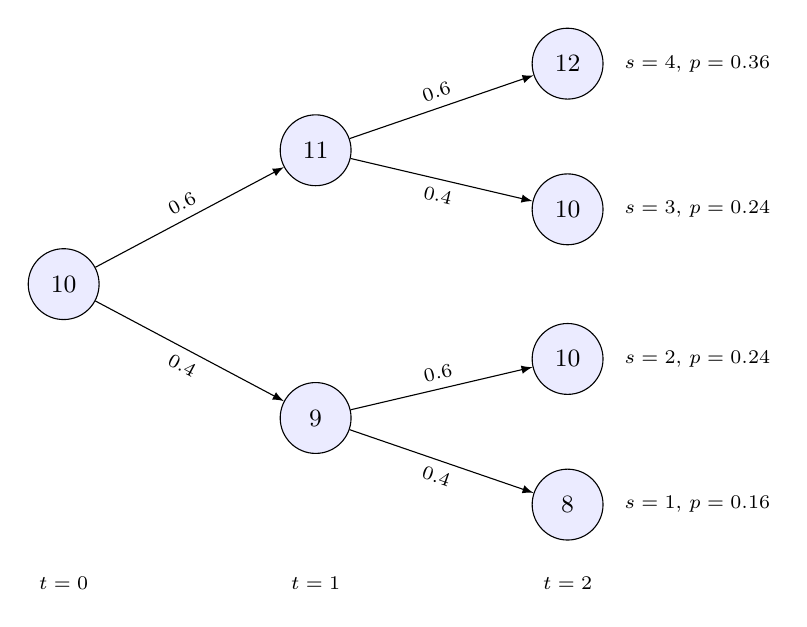
\begin{tikzpicture}[x=1cm,y=1cm,>=latex,font=\small,
  nd/.style={draw,circle,inner sep=1.4pt,minimum size=9mm,fill=blue!8},
  lb/.style={font=\scriptsize,midway,sloped,above}]
  \node[nd] (r)  at (0,0)      {$10$};
  \node[nd] (u)  at (3.2,1.7)  {$11$};
  \node[nd] (d)  at (3.2,-1.7) {$9$};
  \node[nd] (uu) at (6.4,2.8)  {$12$};
  \node[nd] (ud) at (6.4,0.95) {$10$};
  \node[nd] (du) at (6.4,-0.95){$10$};
  \node[nd] (dd) at (6.4,-2.8) {$8$};
  \draw[->] (r)  -- node[lb]{$0.6$} (u);
  \draw[->] (r)  -- node[lb,below]{$0.4$} (d);
  \draw[->] (u)  -- node[lb]{$0.6$} (uu);
  \draw[->] (u)  -- node[lb,below]{$0.4$} (ud);
  \draw[->] (d)  -- node[lb]{$0.6$} (du);
  \draw[->] (d)  -- node[lb,below]{$0.4$} (dd);
  \node[right,font=\scriptsize] at (7.0,2.8)  {$s = 4$, $p = 0.36$};
  \node[right,font=\scriptsize] at (7.0,0.95) {$s = 3$, $p = 0.24$};
  \node[right,font=\scriptsize] at (7.0,-0.95){$s = 2$, $p = 0.24$};
  \node[right,font=\scriptsize] at (7.0,-2.8) {$s = 1$, $p = 0.16$};
  \node[font=\scriptsize,below] at (0,-3.6)   {$t = 0$};
  \node[font=\scriptsize,below] at (3.2,-3.6) {$t = 1$};
  \node[font=\scriptsize,below] at (6.4,-3.6) {$t = 2$};
\end{tikzpicture}
\end{center}

\textbf{(b)(i) Extensive form.} Attach one decision to each \emph{node} of the
tree: $x_0$ at the root, $x_{1,1}$, $x_{1,2}$ at stage 1, and
$x_{2,1}, \ldots, x_{2,4}$ at stage 2, with the states $s$ indexed likewise.
Writing the cost of a node times the probability of reaching it,
\begin{align*}
\min\ & 10x_0
 + 0.4\left(9x_{1,1} + 0.4 \cdot 8 x_{2,1} + 0.6 \cdot 10 x_{2,2}\right)
 + 0.6\left(11x_{1,2} + 0.4 \cdot 10 x_{2,3} + 0.6 \cdot 12 x_{2,4}\right) \\
\text{s.t. } & s_0 = x_0, \\
& s_{1,1} = s_0 + x_{1,1}, \qquad s_{1,2} = s_0 + x_{1,2}, \\
& s_{2,1} = s_{1,1} + x_{2,1}, \quad s_{2,2} = s_{1,1} + x_{2,2}, \quad
  s_{2,3} = s_{1,2} + x_{2,3}, \quad s_{2,4} = s_{1,2} + x_{2,4}, \\
& s_{2,j} = a, \quad j = 1,\ldots,4, \\
& x \geq 0, \quad s \geq 0,
\end{align*}
where node $(1,1)$ carries $\xi_1 = 9$ and node $(1,2)$ carries $\xi_1 = 11$.

\textbf{(b)(ii) Scenario decomposition.} Attach instead one full decision path to
each \emph{scenario}: $x_t^{(s)}$ and $s_t^{(s)}$, $t = 0,1,2$, $s = 1,\ldots,4$.
With $p = (0.16, 0.24, 0.24, 0.36)$ and the cost paths $(10,9,8)$, $(10,9,10)$,
$(10,11,10)$, $(10,11,12)$,
\begin{align*}
\min\ & 0.16\left(10x_0^{(1)} + 9x_1^{(1)} + 8x_2^{(1)}\right)
      + 0.24\left(10x_0^{(2)} + 9x_1^{(2)} + 10x_2^{(2)}\right) \\
& + 0.24\left(10x_0^{(3)} + 11x_1^{(3)} + 10x_2^{(3)}\right)
  + 0.36\left(10x_0^{(4)} + 11x_1^{(4)} + 12x_2^{(4)}\right) \\
\text{s.t. } & s_0^{(s)} = x_0^{(s)}, \quad
 s_t^{(s)} = s_{t-1}^{(s)} + x_t^{(s)}, \quad t = 1,2, \quad s = 1,\ldots,4, \\
& s_2^{(s)} = a, \quad x_t^{(s)} \geq 0, \quad s_t^{(s)} \geq 0, \\
& x_0^{(1)} = x_0^{(2)} = x_0^{(3)} = x_0^{(4)}, & \text{(non-anticipativity, $t=0$)} \\
& x_1^{(1)} = x_1^{(2)}, \qquad x_1^{(3)} = x_1^{(4)}. & \text{(non-anticipativity, $t=1$)}
\end{align*}

\textbf{(c)} Only in the scenario decomposition. The extensive form attaches one
variable per \emph{node}, so two scenarios that are indistinguishable at time $t$
automatically share the same decision: non-anticipativity is built into the
indexing. The scenario decomposition duplicates the decisions along each path,
which is what makes the problem separable by scenario, and the coupling must
then be restored explicitly. Those are precisely the constraints that deck~08
dualizes, with multipliers $\pi$, and that progressive hedging enforces
iteratively.

Note the pattern: at $t = 2$ the four scenarios are all distinguishable, so no
constraint is needed; at $t = 1$ they form two groups; at $t = 0$ a single one.
\end{solution}

%%%%%%%%%%%%%%%%%%%%%%%%%%%%%%%%%%%%%%%%%%%%%%%%%%%%%%%%%%%%%%%%%%%%%%%%%%%%%%
\section{Monte Carlo approximation}
%%%%%%%%%%%%%%%%%%%%%%%%%%%%%%%%%%%%%%%%%%%%%%%%%%%%%%%%%%%%%%%%%%%%%%%%%%%%%%

\begin{exercise}
(Decks~03 and~09.) Show that
\[
\EE_{\bsxi}\left[ \min_{x \in \calX} z(x,\bsxi) \right] \leq \min_{x \in \calX} \EE_{\bsxi}\left[ z(x,\bsxi) \right]
\]
for a deterministic feasible set $\calX$. How is this result to be interpreted
for stochastic programming? Extend it to a Monte Carlo sample average.
\end{exercise}

\begin{solution}
Assume the expectations are well defined and the minima attained, as the
statement implicitly does. There exists $x^* \in \calX$ with
$\min_{x \in \calX} \EE_{\bsxi}[z(x,\bsxi)] = \EE_{\bsxi}[z(x^*,\bsxi)]$. Since
$x^* \in \calX$,
\[
\min_{x \in \calX} z(x,\xi) \leq z(x^*,\xi) \quad \text{for every } \xi,
\]
and taking expectations gives the result.

Without attainment the statement still holds with infima: for every
$y \in \calX$, $\inf_{x \in \calX} z(x,\bsxi) \leq z(y,\bsxi)$, hence
$\EE_{\bsxi}[\inf_{x \in \calX} z(x,\bsxi)] \leq \EE_{\bsxi}[z(y,\bsxi)]$, and
taking the infimum over $y$ closes the argument.

\textbf{Interpretation.} This is $\WSv \leq \RPv$ of deck~03: minimizing under
perfect information is optimistic. A decision tailored to each realization can
only beat a single decision that must serve them all.

\textbf{Extension to sampling.} Let
$z_N(x) = \frac{1}{N}\sum_{n=1}^N z(x,\bsxi_n)$ be the sample average over an
i.i.d.\ sample. The result just proved applies verbatim with the random element
taken to be the whole sample $(\bsxi_1,\ldots,\bsxi_N)$ and the function
$z_N$ in place of $z$:
\[
\EE\left[ \min_{x \in \calX} z_N(x) \right]
\ \leq\ \min_{x \in \calX} \EE\left[ z_N(x) \right]
\ =\ \min_{x \in \calX} \EE_{\bsxi}\left[ z(x,\bsxi) \right],
\]
the last equality because $z_N(x)$ is an unbiased estimator of
$\EE_{\bsxi}[z(x,\bsxi)]$ for each fixed $x$.

\medskip
\emph{Caution.} One cannot argue by exchanging the minimum and the sum, writing
$\min_x \frac{1}{N}\sum_n z(x,\bsxi_n) = \frac{1}{N}\sum_n \min_x z(x,\bsxi_n)$:
the minimum of a sum is not the sum of the minima, and the inequality in fact
runs the other way,
\[
\min_{x \in \calX} \frac{1}{N}\sum_{n=1}^N z(x,\bsxi_n)
\ \geq\ \frac{1}{N}\sum_{n=1}^N \min_{x \in \calX} z(x,\bsxi_n),
\]
since a single $x$ must serve all $N$ draws. That route does not close the chain;
the one above does.

\medskip
The conclusion is that the sample-average optimal value is a
\emph{downward-biased} estimator of the true optimal value: the optimizer
exploits the particular sample it was given. This is the bias that deck~09
analyses, and why an out-of-sample evaluation is needed to obtain an honest upper
bound.
\end{solution}

\end{document}
